\chapter{Обзор литературы}\label{ch:ch1}
\renewcommand{\thefigure}{1.\arabic{figure}} % Plain numbering
\setcounter{figure}{0}                     % Reset if needed
\renewcommand{\figurename}{Рисунок}
%\section{Системы квантовой коммуникации и их применение}\label{sec:ch1/sec1}

\section{Протоколы квантовой коммуникации}\label{sec:ch1/sect2}
Технология квантовой коммуникации позволяет распределить последовательность бит между двумя пользователями,  которым требуется общий ключ для шифрования данных. В отличии от классических методов шифрования, где ключ передается либо специальными службами в случае протоколов симметричного шифрования, или же где ключ состоит из открытой и закрытой части как в методе шифрования RSA. Однако классические системы криптографии имеют ограничения, связанные с их особенностями работы - на сложности математических  вычислений, например факторизации чисел. Однако эта задача может быть решена квантовым компьютером не за полиноминальное время, что представляет угрозу современным способам шифрования.  Есть и другой фактор - необходимость передачи ключа для шифрования и дешифрования информации, переданной между абонентами. 
В качестве решения и было предложено использование технологии квантового распределения ключа. Эта технология позволяет распределять секретный ключ между абонентами с помощью одиночных фотонов. Их использование позволяет перейти к качественно новому уровню передачи ключей, защищенных законами квантовой физики. Из-за этого злоумышленник не может незамеченным считывать квантовые состояния, которыми обмениваются передатчик и приемник, не будучи обнаруженным. Это преимущество вкупе с использованием шифрование методом одноразового блокнота, для которого доказана абсолютная стойкость, ярко выделяет системы квантового распределения ключа среди классических методов шифрования недостижимым уровнем безопасности. 


\subsection{Протоколы квантовой коммуникации на дискретных переменных }\label{sec:ch1/sect2/DVQKD prot}
 В результате исследований, проводившихся по теме квантового распределения ключей, сформировались несколько подходов к реализации протоколов. Первыми протоколами были протоколы на использовании дискретных переменных, в которых для кодирования  используется конечное число дискретных состояний света. Для этого возможно использование одной из двух степеней свободы фотона - фазы или поляризации. Такое подготовленное состояние называется кубитом. Кубит может быть представлен в виде вектора в двхумерном Гильбертовом пространстве как два базовых вектора
\begin{equation}
  \ket{0}       =  \begin{pmatrix} 1 \\ 0 \end{pmatrix}
  \ket{1}       =  \begin{pmatrix} 0 \\ 1 \end{pmatrix}
\end{equation}\label{eq:0 and 1}
Любой кубит может быть представлен как линейная суперпозиция базисов, представленных в выражении \ref{eq:0 and 1}
\begin{equation}
    \ket{\psi}      = \alpha\ket{0} + \beta\ket{1} \&=  cos(\frac{\theta}{2})\ket{0} + e^{i\phi} * sin(\frac{\theta}{2})\ket{1}, 
\end{equation}\label{eq: superpos}
где $\theta \in (0, \pi)$, $\phi \in (0, 2\pi)$, i - мнимая единица. Такое состояние можно изобразить в виде вектора на "Сфере Блоха". В случае $\theta = 0 $ или $\theta = \pi $, получаются состояния $\ket{0}$ и $\ket{1}$ соотвественно. Для векторов, соответствующим значениям фазовым набегам {0, $\frac{\pi}{2}$, $\pi$, $\frac{3\pi}{2}$} получаются следующие вектора:
\begin{equation}
  \phi = 0 : \ket{+}= \frac{1}{\sqrt{2}} \begin{pmatrix} 1 \\ 1 \end{pmatrix}
\end{equation}\label{eq:0 phase vector}
\begin{equation}
  \phi = \pi : \ket{-}= \frac{1}{\sqrt{2}} \begin{pmatrix} 1 \\ -1 \end{pmatrix}
\end{equation}\label{eq:pi phase vector}
\begin{equation}
  \phi/2 = 0 : \ket{+i}= \frac{1}{\sqrt{2}} \begin{pmatrix} 1 \\ i \end{pmatrix}
\end{equation}\label{eq:pi/2 phase vector}
\begin{equation}
  3\phi/2 = 0 : \ket{-i}= \frac{1}{\sqrt{2}} \begin{pmatrix} 1 \\ -i \end{pmatrix}
\end{equation}\label{eq:3pi/2 phase vector}
Полученные векторы описывают дискретные состояния, которые приготавливают для передачи в квантовом канале. Протоколы квантовых коммуникаций, использующие такие типы состояний, называют дискретными. В качестве степеней свободы, в которые кодируется информация, используется как фаза, так и поляризация. При необходимости количество состояний и их значения могут варьироваться, но общая черта - дискретность выбранных значений, не изменяется.
\subsection{Протокол BB84}\label{sec:ch1/sect2/DVQKD prot/bb84 ch1}
Самая первая полноценная работа, посвященная  протоколу квантовой коммуникации, была опубликована в 1984 году, ее авторы Чарльз Беннет и Жиль Брассард\cite{bennett1984a}. По первым буквам их фамилий протокол назван BB84. Эту работу можно считать основополагающей для технологии квантовой коммуникации. 
\newline В классической  криптографии с открытым ключом ловушечные функции используются для скрытия смысла сообщений между двумя пользователями от пассивного подслушивателя, несмотря на отсутствие какой-либо начальной общей секретной информации между двумя пользователями. В квантовом распределении открытых ключей квантовой канал не используется напрямую для отправки осмысленных сообщений, а используется для передачи запаса случайных битов между двумя пользователями, которые изначально не имеют общей секретной информации, таким образом, что пользователи, путем последующей консультации по обычному классическому каналу, который  пассивно подслушивают, могут с большой вероятностью определить, была ли исходная квантовая передача нарушена в пути, как это происходит при подслушивании (преимущество квантового канала в том, что он принуждает подслушивание быть активным). Если передача не была нарушена, они соглашаются использовать эти общие секретные биты известным образом в качестве одноразового блокнота для шифрования смысла последующих осмысленных коммуникаций или для других криптографических приложений (например, аутентификационных тегов), требующих общей случайной информации. Если передача была нарушена, они отбрасывают ее и пытаются снова, откладывая любые осмысленные коммуникации до тех пор, пока им не удастся передать достаточное количество случайных битов через квантовый канал для использования его в качестве одноразового блокнота.
Подробнее, один пользователь ('Алиса') выбирает случайную строку битов и случайную последовательность баз поляризации (прямоугольную или диагональную). Затем она отправляет другому пользователю ('Бобу') поезд фотонов, каждый из которых представляет один бит строки в выбранной для этой позиции бита базе, горизонтальный или 45-градусный фотон означает бинарный ноль, а вертикальный или 135-градусный фотон означает бинарную единицу. По мере того как Боб получает фотоны, он решает, случайным образом для каждого фотона и независимо от Алисы, измерять ли поляризацию фотона в прямоугольной или диагональной базе и интерпретировать результат измерения как бинарный ноль или единицу.  При попытке измерить линейную поляризацию диагонального фотона, или наоборот, генерируется случайный ответ, и вся информация теряется. Таким образом, Боб получает осмысленные данные только от половины фотонов, которые он обнаруживает, те, для которых он угадал правильный базис поляризации. Информация Боба дополнительно ухудшается тем, что, в реалистичном случае, некоторые фотоны будут потеряны в пути или не будут засчитаны не полностью эффективными детекторами Боба. Последующие шаги протокола происходят через обычный общественный канал связи, предполагаемый подверженным подслушиванию, но не внедрению или изменению сообщений. Сначала Боб и Алиса определяют, посредством публичного обмена сообщениями, какие фотоны были успешно получены, и из них, какие были получены в правильном базисе. Если квантовая передача не была нарушена, Алиса и Боб должны согласовать  биты, закодированных этими фотонами, даже если эти данные никогда не обсуждались по общедоступному каналу. Каждый из этих фотонов, другими словами, предположительно несет один бит случайной информации (например, является ли прямоугольный фотон вертикальным или горизонтальным), известный Алисе и Бобу, но никому другому.
Из-за случайной смеси прямоугольных и диагональных фотонов в квантовой передаче любое подслушивание несет риск изменения передачи таким образом, чтобы вызвать рассогласование между Бобом и Алисой по некоторым битам, о которых они считают, что должны сбыть согласованными . В частности, можно показать, что ни одно измерение фотона в пути, сделанное подслушивателем, который узнал о начальной базе фотона только после того, как сделал свои измерения, не может дать более 1/2 ожидаемых битов информации о ключевом бите, закодированном этим фотоном; и что любое такое измерение, давая n битов ожидаемой информации (n $le$ 1/2), должно вызвать несогласие с вероятностью не меньше n/2, если измеренный фотон или его поддельная копия впоследствии будет снова измерена в его начальной базе. (Этот оптимальный компромисс происходит, например, когда подслушиватель измеряет и повторно передает все перехваченные фотоны в прямоугольной базисе, тем самым узнавая правильные поляризации половины фотонов и вызывая несогласия в 1/4 из них, которые позже будут повторно измерены в начальной базе.)
Таким образом, Алиса и Боб могут проверить наличие подслушивания, публично сравнив некоторые биты, по которым они считают, что должны согласиться, хотя, конечно, это пожертвует секретностью этих битов. Позиции битов, использованные в этом сравнении, должны быть случайным подмножеством (скажем, одна треть) правильно полученных битов, чтобы подслушивание более чем нескольких фотонов было маловероятно. Если все сравнения согласуются, Алиса и Боб могут заключить, что квантовая передача была осуществлена без существенного подслушивания, и те из оставшихся битов, которые были отправлены и получены в том же базисе , также согласуются и могут быть безопасно использованы в качестве одноразового блокнота для последующих безопасных коммуникаций по общедоступному каналу. Когда этот одноразовый блокнот будет использован, протокол повторяется для отправки новой порции случайной информации через квантовый канал. Для иллюстрации вышеуказанного протокола далее приводится следующий пример. Необходимость в том, чтобы общественный (не квантовый) канал в этой схеме был защищен от активного подслушивания, может быть смягчена, если Алиса и Боб предварительно договорились о небольшом секретном ключе, который они используют для создания аутентификационных тегов Вегмана-Картера для своих сообщений по общедоступному каналу. Более подробно схема аутентификации множества сообщений Вегмана-Картера использует небольшой случайный ключ для создания зависящего от сообщения "тега" (подобного контрольной сумме) для произвольно большого сообщения таким образом, что подслушиватель, не знающий ключ, имеет только небольшую вероятность создать другие действительные пары сообщение-тег. Тег таким образом предоставляет доказательство того, что сообщение является законным, и не было сгенерировано или изменено кем-то, не знающим ключа. (Биты ключа постепенно исчерпываются в схеме Вегмана-Картера и не могут быть повторно использованы без компрометации доказуемой безопасности системы; однако в данном приложении эти биты ключа могут быть заменены свежими случайными битами, успешно переданными через квантовый канал.) Подслушиватель все еще может предотвратить связь, подавляя сообщения в общедоступном канале, так же как он может подавить или чрезмерно помешать фотонам, отправленным через квантовый канал. Однако в любом случае Алиса и Боб с большой вероятностью заключат, что их секретные коммуникации подавляются, и не будут обмануты, думая, что их связь защищена, когда на самом деле это не так.

\subsection{Протокол B92}\label{sec:ch1/sect2/DVQKD prot/b92 ch1}
В 1992 году Чарльзом Беннетом был предложен альтернативный подход к протоколам квантовой коммуникации \cite{bennett1992}. В \ref{sec:ch1/sect2/DVQKD prot/bb84 ch1} рассматривался протокол, который использует четыре попарно ортогональных, которые находятся в одном базисе, состояния  для кодирования квантовых состояний. В случае же протокола B92 предлагается использование всего двух неортогональных состояний из двух базисов. Благодаря этому протокол Б92 считается одним из самых простейших в реализации за счет использования необходимого  минимума количества состояний для распределения ключа.
\newline Распределение ключей - это термин, применяемый к техникам, позволяющим двум сторонам получить последовательность случайных бит ("ключ") с высоким уровнем уверенности в том, что никто другой не знает его или имеет значительную частичную информацию о нем. Одна сторона (в дальнейшем "Алиса"), например, может сгенерировать ключ с помощью физического случайного процесса, сделать его копию и лично передать копию другой стороне (в дальнейшем "Боб"). Такие общие секретные биты ключа, хотя и случайные, и бессмысленные по себе, являются ценным ресурсом, поскольку позволяют обменивающимся сторонам достичь, с доказанной безопасностью, двух основных целей криптографии: шифрование последующего значимого сообщения, чтобы сделать его непонятным для третьей стороны, и подтверждение легитимному получателю, что сообщение (обычное или зашифрованное) не было изменено в пути.
\newline Если две стороны изначально не обмениваются секретной информацией и общаются исключительно через классические сообщения, которые мониторятся незаконным прослушивателем, для них невозможно получить сертифицированный секретный ключ. Однако это становится возможным, если они обмениваются как классическими публичными сообщениями (которые могут быть мониторены, но не изменены или подавлены прослушивателем), так и квантовыми передачами, которые имеют свойство того, что их можно подавить или изменить, но не могут в принципе быть мониторены без нарушения. Было показано, что различные типы квантовых передач достаточны: случайная последовательность частиц со спином 1/2 или одиночных фотонов в четырех некоординированных поляризационных состояниях (например, в линейной или циркулярной поляризациях); аналогичная случайная последовательность низкоинтенсивных поляризованных когерентных или несогласованных импульсов света; последовательность поляризационно-запутанных состояний Эйнштейна-Подольского-Розена (ЭПР) двухфотонных состояний; и аналогичная последовательность пространственно-временно-запутанных двухфотонных состояний, произведенных, например, параметрической конвертацией. Данный протокол работает следующим образом. 
\begin{enumerate}
    \item \begin{enumerate}
        \item В случае использования ЭПР, Алиса выбирает случайный базис измерений для одного фотона из ЭПР пары: перпендикулярный или циркулярный базис. Другой фотон из пары измеряется Бобом в шаге 3.
    \end{enumerate}
    \item \begin{enumerate}
        \item Измерения Алисы определяют случайную последовательность состояний для фотона Боба: горизонтально поляризованный, вертикально, левоциркулярно или правоциркулярно, через ЭПР-корреляции.
        \item В случае использования ослабленных когерентных состояний, Алиса готовит случайную последовательность фотонов с различными состояниями поляризации: горизонтальной, вертикальной, левоциркулярной или правоциркулярной
    \end{enumerate}
    \item Боб измеряет свой фотон, используя случайную последовательность базисов.
    \item Результаты измерений Боба. Некоторые фотоны не получены из-за неполной эффективности детектора. (Реалистичные детекторы также иногда генерируют ошибки из-за темнвого счета, которые можно обнаружить и исправить.)
    \item Боб сообщает Алисе, какие базисы он использовал для каждого полученного им фотона
    \item Алиса сообщает ему, какие базисы были правильными.
    \item Алиса и Боб оставляют только данные из правильно измеренных фотонов, отбрасывая все остальное
    \item Эти данные интерпретируются как двоичная последовательность в соответствии с кодирующей схемой (0 и 1).
    \item Боб и Алиса проверяют свой ключ, публично выбирая случайное подмножество позиций бит и проверяя, что это подмножество имеет одинаковую четность в версиях ключа у Боба и Алисы (здесь четность нечетная). Если бы их ключи отличались в одной или нескольких позициях бит, эта проверка должна была бы обнаружить этот факт с вероятностью 0.5.
    \item Оставшийся секретный ключ после того, как Алиса и Боб отбросили один бит из выбранного подмножества на шаге 9, чтобы компенсировать информацию, утекшую при раскрытии его четности. Шаги 9 и 10 повторяются k раз, с k независимыми случайными подмножествами, чтобы с вероятностью $1 - 2^{-k}$ удостовериться в том, что ключи Алисы и Боба идентичны, за счет уменьшения длины ключа на k бит. беспокоиться о том, что их ключ был нарушен подслушиванием и должен быть отброшен. 
\end{enumerate}

$1 -\braket{\mu_1}{\mu_2}\neq 0$
Для начала распределения ключа Алиса подготавливает и отправляет Бобу случайную двоичную последовательность квантовых систем, используя состояния ($\ket{u_1}$) и ($\ket{u_2}$), чтобы представлять биты 0 и 1 соответственно. Затем Боб решает, случайным образом и независимо от Алисы для каждой системы, подвергнуть ли ее измерению $P_0$ или $P_1$. Затем Боб сообщает Алисе публично, в каких случаях его измерение дало положительный результат (но, конечно же, не сообщает, какое измерение он сделал), и обе стороны соглашаются отбросить все остальные случаи. Если не было подслушивания, оставшиеся случаи, примерно в доле $(1 -\braket{\mu_1}{\mu_2})/2$ от исходных испытаний, должны быть идеально скоррелированы, состоящими полностью из случаев, когда Алиса отправила ($\ket{u_1}$) и Боб измерил $P_0$, или Алиса отправила ($\ket{u_2}$) и Боб измерил $P_1$. Однако, прежде чем Алиса и Боб смогут доверять этим данным как ключу, они должны, как и в других схемах распределения ключей, пожертвовать некоторую часть для проверки того, что их версии ключа действительно идентичны. Это также удостоверяет отсутствие подслушивания, которое неизбежно нарушило бы состояния ($\ket{u_1}$) или ($\ket{u_2}$) в пути, вызывая иногда положительные результаты при последующих измерениях $P_1$ или $P_0$, соответственно.
\begin{figure}
    \centering
    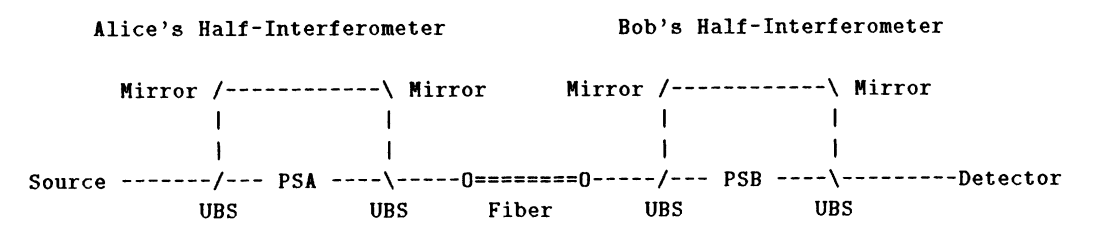
\includegraphics[width=\linewidth]{images/B92 scheme from article.png}
    \caption{Интерферометрическое квантовое распределение ключей с использованием двух неортогональных низкоинтенсивных когерентных состояний. Источник слева поставляет когерентный импульс (волнообразная форма -W-) с интенсивностью ожидаемых фотонов M) 1 в полуинтерферометр Алисы, где несимметричные разделители пучков (UBS), зеркала и фазовый модулятор (PSA 0 или 180 градусов) производят слабый сигнальный импульс (волнообразная форма -w- или, сдвинутый по фазе, -m-), за которым следует яркий опорный импульс -\%-. Отправленные к Бобу через одномодовое оптическое волокно, импульсы входят в полуинтерферометр Боба, где в зависимости от того, является ли сумма фазовых сдвигов Алисы и Боба (PSA+PSB) равной 0 или 180 градусов, сигнальный импульс проходит через верхнее  или нижнее плечо интерферометра и происходит констурктивная или деструктивно интерференция с ослабленным опорным импульсом перед входом в детектор. Перед этим интерференционным импульсом прибывает очень тусклый импульс (не показан), ослабленный как Алисой, так и Бобом, но ни разу не задержанный. После интерференционного импульса прибывает яркий дважды задержанный опорный импульс (волнообразная форма -W-), который Боб контролирует, чтобы убедиться, что опорные импульсы не подавляются. Также не показаны два неиспользуемых пучка, выходящих из правого делителя пучка  каждого полуинтерферометра вниз.}
    \label{fig:B92 sch lit}
\end{figure}
На рисунке \ref{fig:B92 sch lit} показана практическая интерферометрическая реализация, в которой два неортогональных состояния $(\ket{\mu_1})$ и $(\ket{\mu_2})$ представлены слабыми когерентными световыми импульсами, различающимися по фазе относительно сопровождающего яркого эталонного импульса (яркие когерентные состояния, обычно почти ортогональные, становятся значительно неортогональными, когда их ослабляют до ожидаемой интенсивности одного фотона, потому что все такие слабые состояния включают значительную компоненту состояния нулевого количества фотонов). Начиная слева на рисунке, Алиса использует ряд несимметричных делителей пучка и зеркал, чтобы разделить начальный когерентный импульс на два импульса, разделенных во времени: слабый сигнальный импульс интенсивностью p $\neq$ 1 ожидаемый фотон, за которым следует яркий эталонный импульс с M $\neq$ 1 ожидаемым фотоном. Сигнальный импульс сдвигается фазово (PSA) на 0 или 180 градусов для кодирования битов 0 и 1, затем запускается в одномодовое оптическое волокно. Более яркий эталонный импульс не сдвигается по фазе, но задерживается на фиксированное время ht, затем также запускается в то же волокно. На приемном конце аппарата Боб использует полуинтерферометр, аналогичный Алисе, чтобы снова разделить входной пучок, в том же соотношении, что и ранее, на слабую и яркую части. Как и ранее, слабая часть сдвигается по фазе (PSB) на 0 или 180 градусов, случайным образом и независимо от фазовых сдвигов Алисы, в то время как яркая часть задерживается на ht. Наконец, две части приводятся в интерференцию при входе в детектор.
Волна, входящая в детектор, состоит из трех импульсов, разделенных временем $\Delta$t. Первый импульс, очень слабый импульс, который был ослаблен как Бобом, так и Алисой, но не задержан ни одним из них, далее не рассматривается.
Второй импульс, содержащий важную ключевую информацию, представляет собой слабый импульс, состоящий из суперпозиции луча, задержанного Алисой и ослабленного Бобом, и луча, задержанного Бобом и ослабленного Алисой. Если фазовые сдвиги Алисы и Боба равны, произойдет конструктивная интерференция, и суперпозиционный импульс сгенерирует счет с вероятностью, равной $4T_q$ ожидаемых фотонов, где T - коэффициент передачи волокна, а q - квантовая эффективность детектора. Если фазовые сдвиги Алисы и Боба отличаются, интенсивность суперпозиционного импульса будет намного ниже, идеально - ноль в пределе идеального выравнивания интерферометра (время когерентности источника света здесь не имеет значения, поскольку два интерферирующих импульса точно пропорциональны, будучи ослабленными версиями одного и того же исходного импульса).
Наконец, с задержкой $\delta$ t после суперпозиционного импульса к детектору Боба приходит яркий импульс, который был задержан как Алисой, так и Бобом, но не был ослаблен ни одним из них. Боб подтверждает его прибытие, с приблизительной ожидаемой интенсивностью MT, что он может сделать надежно, если M$T_q$) 1. Этот третий импульс не содержит фазовой информации, но служит для подтверждения того, что опорный импульс действительно прибыл. Таким образом, он защищает от атаки, при которой подслушиватель ("Ева") измеряет каждую пару сигнально-опорных импульсов прибором, аналогичным прибору Боба, повторно передает корректно сфабрикованную пару импульсов, когда ей это удается, и подавляет как сигнальный, так и опорный импульсы, когда это не удается, таким образом, подслушивая канал без создания ошибок в последующих результатах измерений Боба. Ива не может подавить опорный импульс без немедленного обнаружения. Но если она подавит только сигнальный импульс, неподавленный опорный импульс все равно вызовет счет в детекторе Боба с вероятностью pTq, и половина этих счетов приведет к ошибкам в ключе Боба.
Кодирование каждого бита в разнице фаз между слабым сигнальным импульсом и сопровождающим его ярким опорным импульсом предоставляет практический способ реализации операторов, аналогичных Po и P~, которые дают гарантированный нулевой результат только для двух законных сигналов ($\mu_i$) и ($\mu_o$), соответственно, но не для фальшивых сигналов (например, вакуумного состояния), которые подслушиватель может подменить. Разделение сигнальных и опорных импульсов по времени также позволяет им передаваться через один и тот же оптический волоконный кабель, что автоматически компенсирует фазовые дрейфы окружающей среды в кабеле, которые в противном случае сделали бы такой большой интерферометр невыполнимым.

Поскольку любая пара когерентных или не когерентных оптических сигналов значительно становится некоординированной при низкой интенсивности, кажется, что почти любой источник двух видов слабых световых вспышек, например, очень ослабленный красный по сравнению с зеленым светофором, можно использовать для распределения ключей без сложностей интерферометрии. Алиса случайным образом отправляет красные и зеленые вспышки с интенсивностью 1 фотон, а Боб публично сообщает, какие вспышки он видел, но не их цвета, которые составляют секретный ключ. Из-за низкой интенсивности Боб может быть уверен, что пассивный злоумышленник, стоящий рядом с ним и наблюдающий за тем же источником сигнала, не увидит того же подмножества импульсов, и, следовательно, будет иметь не всю информацию о ключе, который будет согласован  Алисой. 
Однако более вторженческая Ева, стоящая между Алисой и Бобом, может полностью нарушить схему, перехватывая все вспышки Алисы и пересылая вспышку Бобу только тогда, когда сама видит вспышку Алисы, просто останавливая остальные. Чтобы компенсировать их уменьшенное количество, поддельные вспышки Евы должны быть пропорционально ярче, так чтобы вероятность Боба видеть оставалась той же самой (осторожная Ева должна была бы создавать вспышки с не-Пуассоновской статистикой числа фотонов, чтобы имитировать распределение Пуассона с меньшим средним значением). В терминах формализма операторов проекции, обсуждаемого ранее, схема с красным и зеленым не работает, потому что два сигнала, которые Алиса отправляет здесь, не являются чистыми состояниями, а являются статистическими смесями, в которых фаза электрического поля случайна. Поэтому любой оператор Po, который уничтожает все красные вспышки Алисы, также уничтожит вакуумное состояние, поскольку его можно рассматривать как суперпозицию двух красных вспышек с противоположной фазой. Таким образом, Ева может безопасно заменять вакуумное состояние на любую вспышку, которую она не обнаруживает. В отличие от этого, в интерферометрической схеме на рисунке \ref{fig:B92 sch lit} нет поддельного сигнала, который могла бы подменить подслушивающая сторона, чтобы скрыть свое неудачное обнаружение первоначального сигнала, и схема остается надежной. Эти соображения можно обобщить, чтобы заключить, что распределение ключей возможно не только с использованием любых двух некоординированных чистых состояний ($\mu_n$) и (u ), но и любых двух некоординированных смешанных состояний po и p которые охватывают не пересекающиеся подпространства гильбертова пространства, позволяя Бобу найти два оператора Po и P, таких что Po уничтожает p и P уничтожает $P_0$, но никакое состояние не уничтожается обоими операторами. Требование охвата не пересекающихся подпространств отсутствует в схемах распределения ключей, использующих более двух смешанных состояний, позволяя таким схемам (например, схеме, которая использует четыре некоординированных не когерентных состояния) быть реализованными с помощью простого квадратичного обнаружения оптических сигналов, а не интерферометрического гомодинного обнаружения, как в рисунке \ref{fig:B92 sch lit}

\subsection{Протокол квантовой коммуникации с использованием недоверенного приемного узла} \label{sec:ch1/sect2/MDI QKD}
Существующие протоколы квантовой коммуникации строятся на топологии "точка-точка", в которых участвует всего 2 пользователя: приемник и передатчик. Однако у такого подхода есть уязвимости, связанные  с возможностью злоумышленника контролировать детектор одиночных фотонов, используемого в блоке приемника. Или же использовать другие каналы утечки информации из-за несовершенства детектора одиночных фотонов: различный временной отклик, наличие обратной вспышки при регистрации фотона. Как решение всех известных уязвимостей детекторов одиночных фотонов был разработан протокол КРК с недоверенным приемным узлом (НПУ-КРК) или же Measurement-Device-Independent Quantum Key Distribution (MDI-QKD). 
\newline В данной работе представлена идея квантовой криптографии с измерениями, независимыми от устройства (MDI-QKD) \cite{lo2012,liu2013}, как простое решение для устранения всех (существующих и еще не обнаруженных) каналов утечки информации, связанных с детектором \cite{zhao2008}, пожалуй, самой критической части реализации, и показываем, что у нее как отличные показатели безопасности, так и производительности. Таким образом, она предлагает огромное преимущество в безопасности по сравнению со стандартными доказательствами безопасности, такими как доказательства Инамори-Люткенхауса-Майерса (ILM) \cite{inamori2007} и Готтесмана-Ло-Люткенхауса-Прескилла (GLLP). \cite{gottesman2004} Более того, данный подход позволяет удвоить дальность передачи, которую могут покрыть те схемы квантовой криптографии, которые используют обычные полупроводниковые лазеры, а ее скорость генерации ключей сравнима со стандартными доказательствами безопасности с использованием запутанных пар. В отличие от квантовой криптографии с прямыми измерениями (DI-QKD), в ее простейшей формулировке MDI-QKD требует дополнительного предположения о том, что у Алисы и Боба почти идеальная подготовка состояний. Однако это не препятствие, потому что источники сигнала Алисы и Боба могут быть ослабленными лазерными импульсами, подготовленными ими самими. Их состояния могут быть экспериментально проверены в полностью защищенной лабораторной среде за пределами вмешательства Евы через случайную выборку. Более того, как будет обсуждаться позже, недостатки в процессе подготовки Алисы и Боба на самом деле могут быть легко устранены в более точной формулировке протокола.
\newline Простой пример нашего метода следующий. Как Алиса, так и Боб подготавливают слабые когерентные импульсы (СКИ) с фазовым кодированием в четырех возможных поляризационных состояниях BB84 (т. е. вертикальном, горизонтальном, поляризованном под углом 45 и 135 градусов) \cite{bennett1984} и отправляют их ненадежному ретранслятору Чарли (или Еве), находящемуся посередине, который выполняет измерение состояния Белла, проецирующее входные сигналы в состояние Белла. Такое измерение может быть реализовано, например, с использованием только линейных оптических элементов с установкой, показанной на рисунке \ref{fig:MDI scheme lit} (На самом деле, такая установка определяет только два из четырех состояний Белла. Но это не проблема, поскольку любое состояние Белла позволяет доказать безопасность.) Кроме того, Алиса и Боб применяют методы фальшивых состояний, чтобы оценить усиление (т. е. вероятность успешного результата ретранслятора) и квантовую погрешность бита (QBER) для различных чисел входных фотонов. После завершения квантовой коммуникационной фазы Чарли использует открытый канал для объявления событий, где он получил успешный результат в ретрансляторе, а также свой результат измерения. Алиса и Боб сохраняют данные, соответствующие этим случаям, и отбрасывают остальные. Кроме того, как и в BB84, они на этапе постобработки выбирают события, где они используют тот же базис в своей передаче с помощью аутентифицированного открытого канала. Наконец, чтобы гарантировать, что их битовые строки правильно коррелируются, Алиса или Боб должны применить инверсию бита к своим данным, за исключением случаев, когда они оба выбирают диагональную базу и Чарльз получает успешный результат измерения, соответствующий тройному состояний. Давайте теперь подробно оценим производительность протокола выше. Для простоты рассматривается улучшенный анализ данных, при котором Алиса и Боб оценивают данные, отправленные в двух разных базисах \cite{lo2005}. В частности, используется линейный базис в качестве базиса генерации ключей, в то время как диагональный базис используется только для тестирования.
\begin{figure}
    \centering
    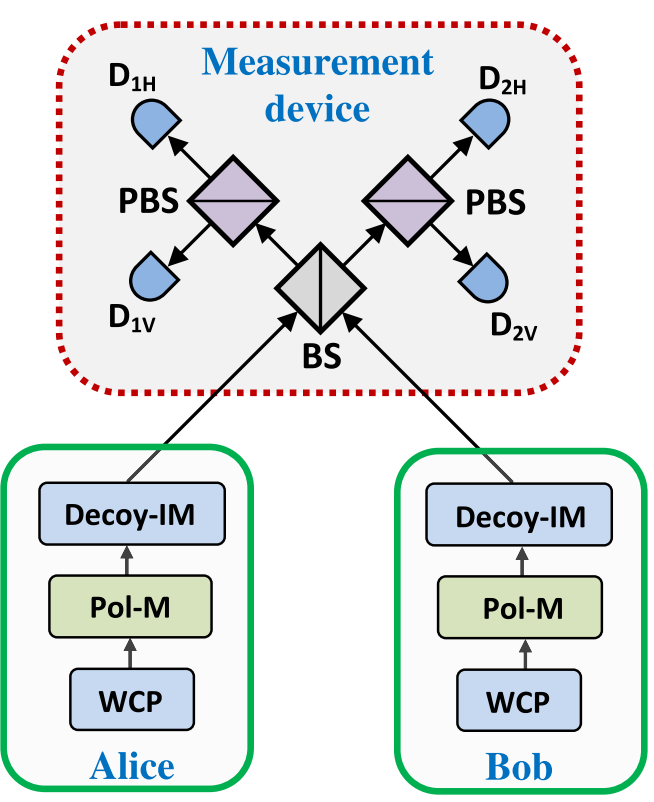
\includegraphics[width=0.7\linewidth]{images/MDi scheme.png}
    \caption{Базовая схема протокола MDI-QKD.
Алиса и Боб подготавливают фазово случайные слабые когерентные импульсы (СКИ) в разных поляризационных состояниях BB84, которые выбираются независимо и случайным образом для каждого сигнала с помощью модулятора поляризации (Pol-M). Состояния - ловушки генерируются с использованием модулятора интенсивности (Decoy-IM). Внутри измерительного устройства сигналы от Алисы и Боба интерферируют на светоделителе  (BS) с коэффициентом деления 50:50, на каждом конце которого находится поляризационный светоделитель (PBS), направляющий входящие фотоны в горизонтальные (H) или вертикальные (V) поляризационные состояния. Четыре фотодетектора используются для обнаружения фотонов, и результаты обнаружения объявляются публично. Успешное измерение состояния Белла соответствует наблюдению активации ровно двух детекторов (связанных с ортогональными поляризациями). Клик в $D_{1H}$ и $D_{2V}$ или в $D_{1V}$ и$D_{2H}$ указывает на проекцию на состояние Белла $\ket{\psi^{-}} = \frac{1}{\sqrt{2}}(\ket{HV} - \ket{VH})$, в то время как клик в $D_{1H}$ и $D_{1V}$ или в $D_{2H}$ и $D_{2V}$ показывает проекцию на состояние Белла $\ket{\psi^{+}} = \frac{1}{\sqrt{2}}(\ket{HV} + \ket{VH})$. Установки Алисы и Боба надежно защищены от прослушивателя, в то время как измерительное устройство может быть ненадежным.
}
\end{figure} \label{fig:MDI scheme lit}
\newline Для обзоначений введем $Q_{rect}^{n,m} , Q_{diag}^{n,m} , e_{rect}^{n,m} , e_{diag}^{n,m}$ - обозначают, соответственно, усиление и QBER сигнальных состояний, отправленных Алисой и Бобом, где n и m обозначают количество фотонов, отправленных законными пользователями, а rect или diag представляет их выбор базиса.
\newline (A) Прямоугольный базис. Ошибка соответствует успешному выводу ретранслятора, когда и Алиса, и Боб подготавливают одно и то же поляризационное состояние (т. е. их результаты должны быть антикоррелированы до применения инверсии бита). Предполагая на данный момент идеальные оптические элементы и детекторы, и отсутствие смещения, имеем, что каждый раз, когда Алиса и Боб отправляют, соответственно, n и m фотонов, подготовленных в одном и том же поляризационном состоянии, ретранслятор никогда не выдаст успешный результат. Таким образом, получаем, что $e_{rect}^{n,m}$
 равно нулю для всех n, m. Это означает, что для отфильтрованного ключа не требуется коррекция ошибок. Это замечательно, потому что это подразумевает, что использование источников СКИ (вместо однофотонных источников) не существенно снижает скорость генерации ключей протокола квантовой криптографии (в части коррекции ошибок).
\newline (B) Диагональный базис. Чтобы определить количество необходимой амплификации конфиденциальности, рассматривается диагональный базис. Ошибка соответствует проекции на синглетное состояние в случае, когда Алиса и Боб подготавливают одно и то же поляризационное состояние, или на тройное состояние, когда они подготавливают ортогональные поляризации. Предполагая опять же идеальный сценарий, обсуждаемый в предыдущем абзаце, находим, что $e_{diag}^{1,1}$ = 0. (Это происходит потому, что когда два идентичных однофотонных входят в 50:50 светоделитель, эффект Хонга-Оу-Манделя \cite{hong1987} гарантирует, что оба фотона всегда выйдут из светоделителя вместе в том же самом выходном режиме. Кроме того, если два фотона подготовлены в ортогональных поляризациях и они выходят из 50:50 светоделителя в том же самом выходном плече, оба фотона всегда достигнут одного и того же детектора внутри ретранслятора.) Тот факт, что $e_{diag}^{1,1}$ равно нулю, вновь поразителен, так как это означает, что использование источников СЦИ существенно не снижает скорость генерации ключей (также в части усиления секретности).
\newline (C) Скорость генерации ключей. В идеальном сценарии, описанном выше, скорость генерации ключей будет просто определяться как $R = Q_{rect}^{1,1}$ в асимптотическом пределе бесконечно длинного ключа. С другой стороны, если учитываются недостатки, такие как смещение базиса и темные отсчеты, скорость генерации ключей в реалистичной настройке будет определяться как
\begin{align}
    R = Q_{rect}^{1,1}[1-H(e_{diag}^{1,1})] - Q_{rect}f(E_{rect})H(E_{rect})
\end{align} \label{eq:MDI key rate},
где $Q_{rect}$ и $E_{rect}$ обозначают, соответственно, усиление и QBER в прямоугольном базисе ( то есть $  Q_{\text{rect}} = \sum_{n,m} Q_{\text{rect}}^{n,m}  $ и $E_{\text{rect}} =\sum_{n,m} \frac{Q_{rect}^{n,m}e_{rect}^{n,m}}{Q_{rect}}$, $\text{f}(E_{rect}) > 1$ функция неэффективности для процесса коррекции ошибок, а $H\text{(x)} = - x\log_2(x) - (1 - x)\log_2(1-x) $  функция бинарной энтропии Шеннона. Есть несколько нерешенных вопросов, которые нужно прояснить. Во-первых, предполагается, что метод фальшивых состояний можно использовать для оценки усиления $Q_{rect}^{1,1}$ и QBER $e_{rect}^{1,1}$. 
\begin{figure}
    \centering
    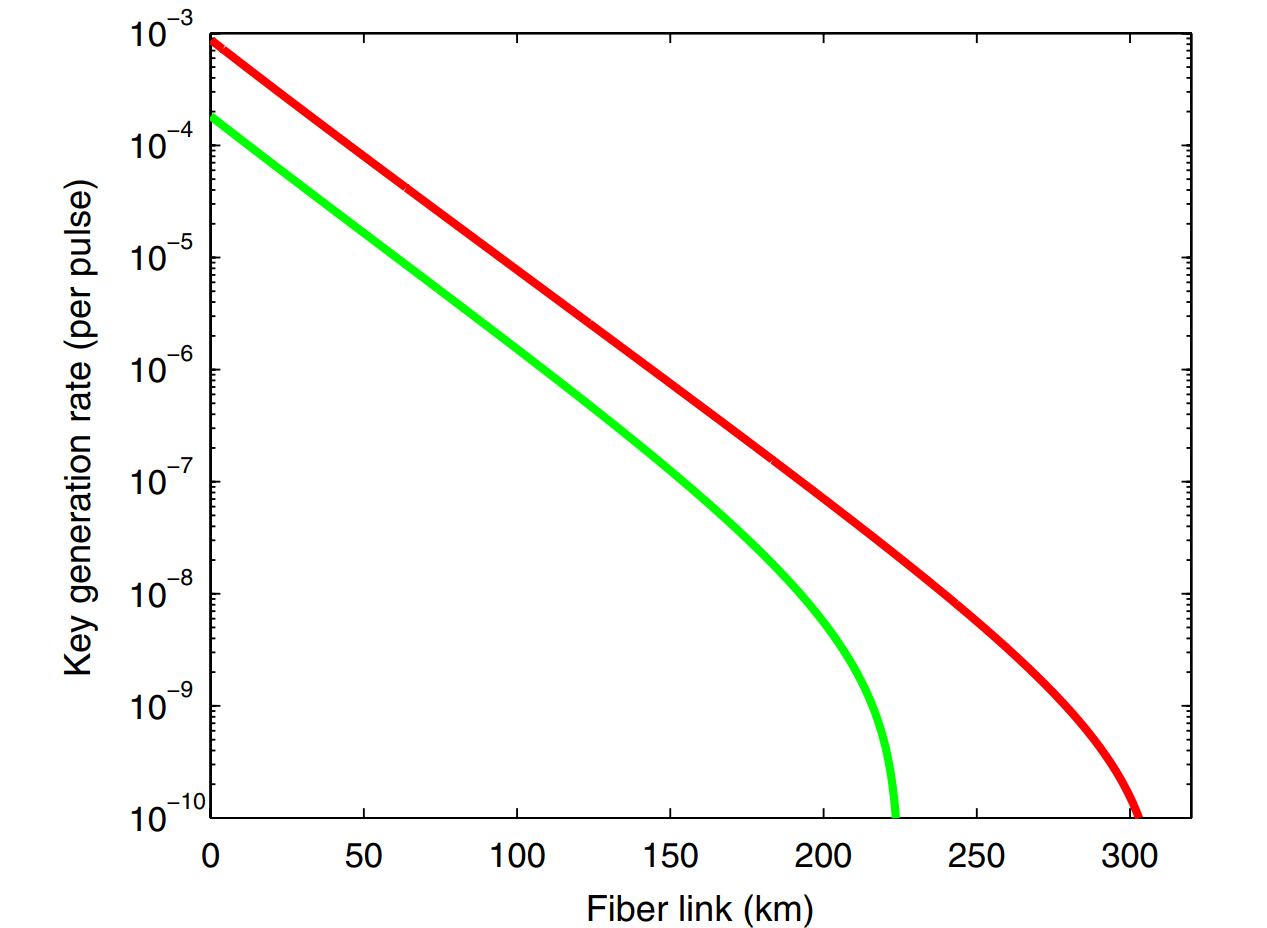
\includegraphics[width=0.8\linewidth]{images/mdi speed.png}
    \caption{Нижняя граница секретной скорости ключа R, заданная уравнением \ref{eq:MDI key rate}, в логарифмической шкале для установки MDI-QKD с использованием слабых когерентных импульсов, показанной на рисунке \ref{fig:MDI scheme lit} (зеленая кривая). В целях моделирования рассматриваются следующие экспериментальные параметры: коэффициент потерь канала составляет 0,2 дБ/км, внутренняя ошибка из-за смещения и нестабильности оптической системы составляет 1,5\%, эффективность обнаружения реле (т. е. пропускная способность его оптических компонентов вместе с эффективностью его детекторов) составляет 14,5\%, а фоновая частота счета составляет 6,02 × $10^(-6)$. (Для простоты рассматривается упрощенную модель смещения, помещая унитарное вращение в одну из входных ветвей светоделителя с делением пополам 50:50 и также унитарное вращение в одну из его выходных ветвей. Общее значение смещения составляет 1,5\%. То есть, мы предполагаем смещение в 0,75\% в каждом вращении.) В сравнении красная кривая представляет нижнюю границу R для протокола квантовой криптографии на основе запутанных пар с источником на основе параметрического преобразования с понижением частоты (PDC), расположенным посередине между Алисой и Бобом \cite{ma2007}. На красной кривой предполагается, что используется оптимальная яркость источника PDC. Однако на практике яркость источника PDC ограничена технологией. Поэтому скорость ключа протокола квантовой криптографии на основе запутанных пар будет значительно ниже, чем показано на красной кривой. Это делает наше новое предложение еще более привлекательным по сравнению с существующими данными на рисунке}
\end{figure} \label{fig:key rate MDI lit}
Во-вторых, нам нужно оценить секретную скорость ключа, заданную уравнением \ref{eq:MDI key rate}, для реалистичного устройства 
Во-вторых, нам нужно оценить секретную скорость ключа, заданную уравнением \ref{eq:MDI key rate}, для реалистичной настройки. Давайте уточним эти моменты здесь. Действительно, можно показать, что метод оценки соответствующих параметров в формуле для скорости ключа эквивалентен используемому в стандартных системах квантовой криптографии с фальшивыми состояниями. Для целей моделирования рассматриваются неэффективные и шумные пороговые детекторы и используем экспериментальные параметры из \cite{takeoka2014} за исключением того, что \cite{takeoka2014} рассматривает канал свободного пространства, тогда как здесь рассматривается канал на основе оптоволокна с потерей 0,2 дБ/км. Более того, для простоты предполагается, что все детекторы идентичны (т.е. у них одинаковая частота темных отсчетов и эффективность обнаружения), и их темные отсчеты, приблизительно, независимы от входящих сигналов. Кроме того, используется протокол коррекции ошибок с функцией неэффективности $\text{f}(E_{rect})$ = 1,16 \cite{pirandola2017}. Полученная нижняя граница секретной скорости ключа проиллюстрирована на рисунке \ref{fig:TF key rate lit}. Наши расчеты и результаты моделирования показывают, что скорость генерации ключей существенно сравнима с доказательством безопасности \cite{ma2007} для протоколов квантовой криптографии на основе запутанных пар. Наша схема может выдерживать высокие оптические потери более 40 дБ или 200 км ВОЛС, если ретранслятор размещается посередине между Алисой и Бобом. Другими словами, можно практически удвоить дистанцию передачи по сравнению с установкой, где аппарат измерения состояния Белла находится у Алисы, или установкой с использованием стандартного протокола BB84 с фальшивыми состояниями.
Чтобы экспериментально реализовать предложенный протокол MDI-QKD, несколько практических вопросов требуют решения. Среди них, возможно, самый важный - это то, как генерировать неразличимые фотоны из двух независимых лазерных источников и наблюдать стабильное интерференционное явление Хонга-Оу-Манделя \cite{hong1987}. Обратите внимание, что физика, лежащая в основе этого протокола, основана на явлении группировки фотонов в одну группу двух неразличимых фотонов на 50:50 светоделителе. Здесь проводится простой эксперимент принципиального доказательства, чтобы показать, что высокая видимость интерференции Хонга-Оу-Манделя между двумя независимыми лазерами, которые возможно приобрести, вполне осуществима. Результаты показаны на рисунке \ref{fig:TF key rate lit}. Согласованность между экспериментальными и теоретическими результатами подтверждает, что высокая видимость интерференционного провала Хонга-Оу-Манделя может быть достигнута даже с двумя независимыми лазерами.
Идею MDI-QKD можно обобщить намного дальше. Во-первых, она также применима в случае, когда Алиса и Боб используют запутанные пары фотонов в качестве источников. Во-вторых, она работает даже в том случае, когда процессы подготовки Алисы и Боба неидеальны. Действительно, зависимость от базиса, возникающая из недостатка в процессах подготовки Алисы и Боба, может быть легко устранена с помощью идеи квантовой монетки \cite{gottesman2004,koashi2005}, чтобы количественно оценить количество зависимого от базиса недостатка \cite{tamaki2012}. В-третьих, заметим, что в практических приложениях потребуется только конечное количество фальшивых состояний. Это аналогично стандартным протоколам квантовой криптографии с конечными фальшивыми состояниями \cite{ma2005}, которые широко используются в экспериментах \cite{rosenberg2009}. В-четвертых, MDI-QKD работает даже без уточненного анализа данных. В-пятых, она также работает для других протоколов квантовой криптографии, включая протокол из шести состояний \cite{fuchs1997}. Эти вопросы, вместе с учетом эффектов конечного размера, возникающих потому, что Алиса и Боб отправляют только конечное количество сигналов в каждом запуске протокола квантовой криптографии\cite{tamaki2012}.

В заключение, предлагается идея квантовой криптографии с измерительно-устройствонезависимым подходом (MDI-QKD). По сравнению со стандартными доказательствами безопасности, у него есть ключевое преимущество в удалении всех каналов боковых сигналов детектора, и он может удвоить дистанцию передачи, охватываемую с помощью обычных протоколов квантовой криптографии с использованием слабых когерентных импульсов. Более того, у него довольно высокая скорость генерации ключей, которая сравнима с таковой в стандартных доказательствах безопасности. Действительно, его скорость генерации ключей на порядки выше, чем предыдущий подход полностью измерительно-устройствонезависимой квантовой криптографии. Нашу идею можно реализовать с помощью стандартных пороговых детекторов с низкой эффективностью обнаружения и каналов с высокими потерями. Учитывая его отличную безопасность, производительность и простую реализацию, считается что MDI-QKD является большим шагом вперед в сокращении разрыва между теорией и практикой квантовой криптографии, и ожидаем, что он будет широко применяться в практических системах квантовой криптографии в будущем.
\subsection {Протокол квантовой коммуникации с использованием полей близнецов}\label{sec:ch1/sect2/TF QKD lit}
Значительный теоретический прогресс в достижении практического безопасного QKD на больших расстояниях был достигнут с предложением QKD с двойным полем (TFQKD)\cite{scarani2009}, которое улучшает масштабирование ключевой скорости в соответствии с квадратным корнем из пропускания канала. Он показывает, что источник когерентного состояния на самом деле может быть преимуществом по сравнению с однофотонным источником, поскольку постселекция фазовой когерентности двойных полей Алисы и Боба может потенциально привести к безопасному QKD с кодирующим состоянием одного фотона и вакуума, а также их линейных суперпозиций. Этот метод способен достичь скорости передачи ключей, зависящей от квадратного корня из коэффициента пропускания канала, и, таким образом, преодолеть известное ограничение по расстоянию для существующих протоколов практического QKD. Теоретически безопасная ключевая скорость может быть даже выше, чем возможности секретных ключей без ретрансляторов, известные как границы Такеока-Гуха-Вильде \cite{takeoka2014} и Пирандола-Лауренца-Оттавиани-Бьянки (PLOB) \cite{pirandola2017}. Однако для того, чтобы сделать это реальностью, еще предстоит проделать значительную работу. Во-первых, существует теоретическая проблема объединения постселекции фазовой информации с традиционным методом ложных состояний. Во-вторых, это технически сложная задача точной интерференции одиночных фотонов на большом расстоянии. Для достижения этой цели был предложен протокол "посылать или не посылать" (SNS) \cite{wang2018}. Он предполагает малые вероятности отправки для Алисы и Боба, а затем использует решения об отправке и отказе от отправки для кодирования битовых значений в базисе Z с эффективными событиями-вестниками, объявляемыми Чарли. Таким образом, как было показано в \cite{wang2018}, в протоколе можно продолжать использовать модель с метками и обычный метод ложных состояний. Кроме того, поскольку протокол кодирует битовые значения, используя почти безошибочный базис Z, он может терпеть высокую частоту ошибок в базисе X. 
\begin{figure}
    \centering
    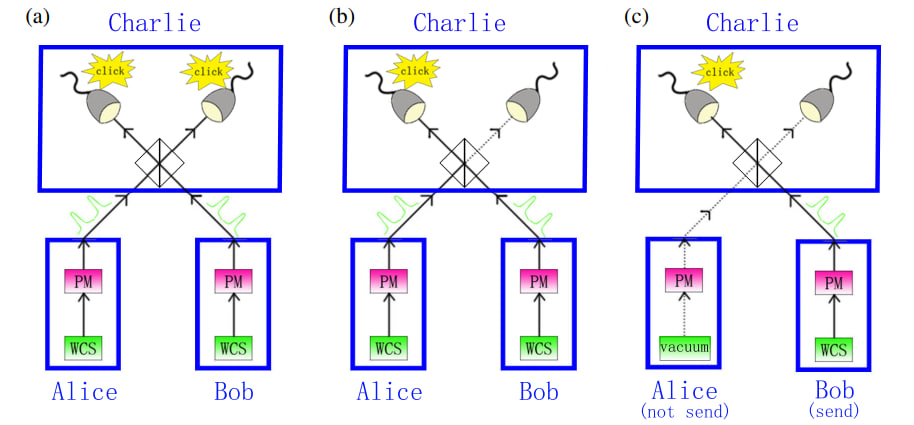
\includegraphics[width=\linewidth]{images/TF schemes lit.jpg}
    \caption{Схемы трех различных протоколов. (a) MDIQKD с состояниями-ловушками, где пары импульсов с когерентным состоянием в кодировке BB84 рассылаются, а эффективные события предвещаются двукратным срабатыванием. Скорость передачи ключей линейно зависит от пропускания канала. (b) Оригинальное состояние приманки TFQKD \cite{lucamarini2018}, в котором сдвоенные поля когерентных состояний со случайными фазовыми сдвигами посылаются по базам X и Y, а эффективные события возвещаются одиночным щелчком. Скорость передачи ключей зависит от квадратного корня из пропускания канала. Для обоих базисов необходимы однофотонные помехи от удаленных независимых источников. Возможны ошибки рассогласования в обеих базах, и информация о фазовом сдвиге после объявления делает метод "приманка-состояние" недействительным. (c) SNSTFQKD (Sending - not sending TFQKD) с состояниями ловушками \cite{ma2005}. В базисе Z каждая сторона независимо принимает решение об отправке с небольшой вероятностью. События, когда одна сторона решает отправить, другая сторона решает не отправлять, и один и только один детектор щелкает (как показано на рисунке), являются целевыми событиями для генерации защищенных ключей. Он отказоустойчив к большой ошибке смещения в базисе X, так как ошибка смещения в базисе Z отсутствует. Традиционный метод "приманка-состояние" работает, поскольку информация о фазовом сдвиге в базисе Z никогда не объявляется. Объявление одного щелчка делает эффективными события в базисе Z, а ключевая скорость находится в масштабе квадратного корня из пропускания канала. WCS: слабый когерентный источник}
    \label{fig:TF protocols scheme}
\end{figure}
В этой работе рассматривается экспериментальная демонстрация КРК с полями-близнецами через протокол SNS (SNSTFQKD) по катушкам оптического волокна.
Протокол.- Рассмотрим схему протокола SNSTFQKD \cite{ma2007}, показанную на рисунке \ref{fig:TF protocols scheme}. Здесь реализуется протокол с помощью практического метода четырех интенсивностей \cite{gobby2004}, где каждая сторона использует четыре различные интенсивности, а именно 0, $\mu_1$, $\mu_2$ и $\mu_z$. Алиса и Боб случайным образом выбирают базис X или Z с вероятностями pX и 1 - pX, соответственно. В базисе X Алиса и Боб готовят и посылают импульсы-обманки. Фазовые сдвиги $\theta_A$ и $\theta_B$ частным образом накладываются на их импульсы. Событие в базисе Z считается эффективным, если Чарли объявляет, что щелкнул только один детектор. Для того чтобы событие X-базиса было эффективным, нам необходимо дополнительное условие фазового среза, чтобы уменьшить наблюдаемую частоту ошибок в базисе. Без разумного условия фазового среза наблюдаемый коэффициент ошибок в базисе X может быть слишком большим, чем фактический коэффициент ошибок в базисе Z. Обратите внимание, что Чарли не обязан быть честным, и все, что он объявляет, не подрывает безопасность. Но если Чарли хочет получить высокую скорость генерации секретного ключа, ему придется постараться сделать правдивое объявление обо всем. Ошибка в базисе X определяется как объявление Чарли о щелчке правого (левого) детектора, связанном с эффективным событием в базисе X, когда разница фаз между парой импульсов от Алисы и Боба, вероятно, вызвала бы щелчок слева (справа) на измерительной установке Чарли. Эффективное событие в базисе Z, которое Алиса (Боб) решила отправить, а Боб (Алиса) решил не отправлять, соответствует значению бита 1 (0). Значения $\epsilon_1^{ph}$ и $s_1$, выход однофотонных эффективных событий в базисе Z, могут быть рассчитаны обычным методом ложных состояний.
\begin{figure}
    \centering
    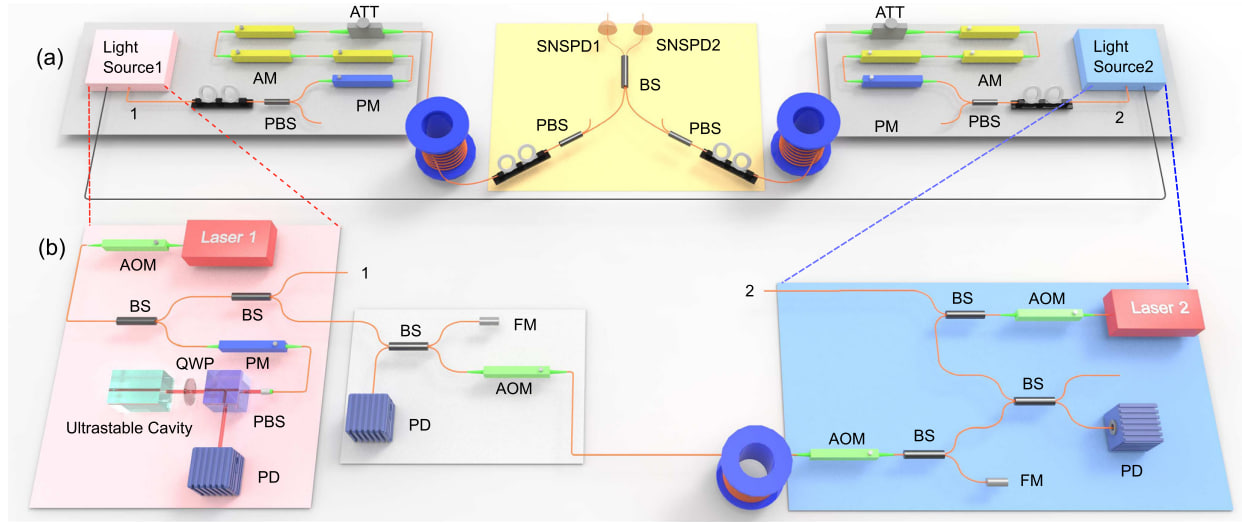
\includegraphics[width=\linewidth]{images/TF experiment scheme.jpg}
    \caption{(a) Схема нашей экспериментальной установки. В качестве источников Алиса и Боб используют непрерывный лазер с частотной синхронизацией.  Эти лазеры затем модулируются фазовым модулятором (ФМ) и тремя амплитудными модуляторами (АМ) для рандомизации фазы, кодирования и модуляции интенсивности обманки. Затем импульсы ослабляются аттенюатором (ATT) и отправляются по оптоволоконным катушкам к Чарли. На измерительной станции Чарли На измерительной станции Чарли импульсы от Алисы и Боба проходят через поляризационные контроллеры (PC) и поляризационные разветвители луча (PBS), затем интерферируют на разветвителе луча (BS). Наконец, свет измеряется сверхпроводящими нанопроволочными однофотонными детекторами (SNSPD). (b) Система частотной синхронизации для лазеров Алисы и Боба. Длина волокна между Алисой и Бобом установлена равной общей длина сигнального волокна. AOM: акустооптический модулятор, FM: зеркало Фарадея, PD: фотодиод. QWP: четвертьволновая пластина.}
    \label{fig:TF experiment scheme}
\end{figure}
Схема эксперимента показана на рисунке \ref{fig:TF experiment scheme}(a). В установках Алисы и Боба в качестве источников света используются независимые лазеры с непрерывной волной (cw). Свет модулируется на 16 различных фаз с помощью фазового модулятора (ФМ) и кодируется с помощью трех амплитудных модуляторов (АМ). В эксперименте устанавливается базовый период 5 мкс, в течение которого в первые 3 мкс посылается 100 сигнальных импульсов с шириной импульса 2 нс и интервалом 30 нс, затем в следующие 1,2 мкс - 4 фазовых опорных импульса для оценки относительной фазы между каналами Алисы и Боба, и в заключительные 0,8 мкс - состояние вакуума в качестве времени восстановления сверхпроводящих нанопроволочных однофотонных детекторов (SNSPDs). Интенсивности сигналов устанавливаются в оптимизированные состояния приманки $\mu_z$, $\nu_1$, $\nu_2$ или 0 . Затем сигналы передаются от Алисы и Боба к Чарли, где они интерферируют. Поскольку для интерференции требуются идентичные входные сигналы, для компенсации поляризационного дрейфа канала необходимы поляризационные контроллеры (PC) и поляризационные разветвители луча (PBS) перед поляризационными поддерживающими разветвителями луча (BS). Результаты интерференции затем обнаруживаются с помощью SNSPD и регистрируются с помощью высокоскоростного устройства регистрации времени. Основной технической проблемой при реализации SNSTFQKD является управление фазовой эволюцией полей-близнецов. Как было указано в, дифференциальное колебание фазы между двумя пользователями может быть записано как
\begin{align}
    \delta_{ba} = \frac{2\pi}{s}(\delta\nu L + \nu\delta L)
\end{align}\label{eq: TF phase fluct lit},
 где $\nu$- оптическая частота света, L - длина волокна, s - скорость света в волокне. Таким образом, необходимо компенсировать два источника, вносящих вклад в разность фаз: первый член в уравнении обозначает разность частот между Алисой и Бобом, а второй - дрейф фазы в волокне. В качестве примера, измеренная скорость дрейфа фазы соответствует гауссову распределению со стандартным отклонением 7,4 рад $мс^{-1}$ для общего расстояния волокна 150 км. Чтобы справиться с разницей фаз, вызванной разницей длин волн, используется метод частотной синхронизации, как показано на рисунке \ref{fig:TF experiment scheme}(b). В лаборатории Алисы в качестве начального лазера используется лазер непрерывной волны с центральной длиной волны 1550,12 нм и шириной линии в несколько килогерц. Начальный лазер фиксируется в ультрастабильном резонаторе длиной 10 см с тонкостью около 250 000 с помощью техники Паунда-Древера-Холла, чтобы подавить его ширину линии с нескольких килогерц до примерно десяти герц. Затем свет разделяется на две части, одна из которых используется в качестве источника Алисы, а другая - для блокировки оптической частоты Боба. Этот блокирующий луч далее разделяется на две части, одна из которых отражается от зеркала Фарадея (FM) в качестве локального эталона, а другая частотно-модулируется акустооптическим модулятором (AOM) и отправляется Бобу. Здесь длина волокна установлена равной расстоянию передачи сигнала, чтобы продемонстрировать практичность системы.

 Вместо того чтобы активно стабилизировать относительную фазу между Алисой и Бобом, разница фаз компенсируется с помощью постобработки. Определив оценочную относительную фазу между волокнами Алисы и Боба как $\Delta\phi_T$, вычисляется квантовый коэффициент битовых ошибок в базисе X для обнаружений, лежащих в диапазоне 
 \begin{align}
    1 - |\cos(\theta_A - \theta_B + \delta\phi_T| < \Lambda)
\end{align}\label{eq: QBER error TF}
 где $\theta_A (\theta_B)$ - случайная фаза, которой Алиса (Боб) модулирует сигнал, а $\Lambda$ - заданный диапазон. Тогда вычислить безопасную ключевую скорость с эффектом конечного размера данных по следующей формуле:
 \begin{align}
    R = (1 - p_x)^2{2p_z(1-p_z)a_1s_1[1 - H(e_1^{ph})] - fS_zH(E_z)} - \frac{1}{N_{total}}log_2\frac{1}{\epsilon^5}
\end{align}\label{eq: TF qkd rate lit}
 где R - конечная ключевая скорость, $a_1 = \mu_{\zeta}e^{-\mu_{\zeta}}$, $s_1$ - выход эффективных однофотонных событий в базисе Z, $\epsilon_1^{ph}$ - коэффициент фазовой ошибки для событий в базисе Z, $S_Z$ и $E_Z$ - наблюдаемый выход и коэффициент битовой ошибки для базиса Z, $N_{total}$ - общее число посланных сигнальных импульсов, а $\epsilon =10^{-10}$, что соответствует общей вероятности отказа $2*10^{-9}$. Скорость передачи ключей была бы еще выше, если бы мы учитывали только статистические флуктуации. Здесь предполагается, что эффективность исправления ошибок составляет f = 1.1. В работе протестирован SNSTFQKD с общим расстоянием между Алисой и Бобом от 0 до 300 км.  Во всех экспериментах с различными длинами волокон общее количество импульсов, посылаемых Алисой и Бобом, установлено на уровне $7.2*10^{11}$. Достоверные детектирования составляют $6.5*10^{9}$, $2.3*10^{9}$2,3 × 109, $7.6*10^{8}$ и $2.5*10^{9}$ для 0, 50, 100 и 150 км в первом эксперименте и $1.7*10^{9}$, $1.9*10^{8}$  и  $2.4*10^{7}$ для 100, 200 и 300 км во втором эксперименте. 
 \begin{figure}
     \centering
     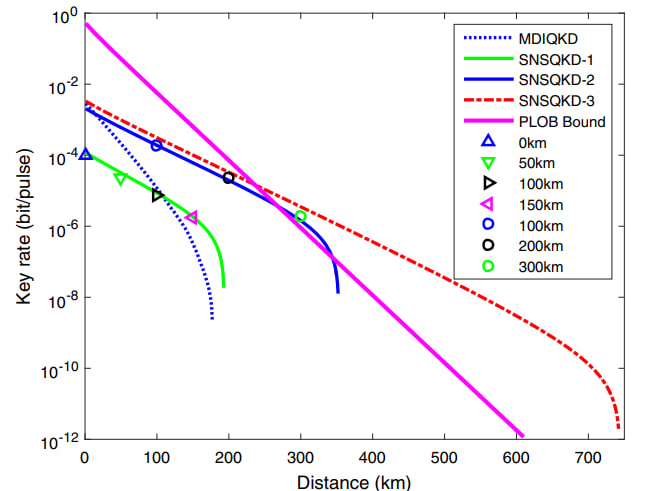
\includegraphics{images/TF key rate lit.jpg}
     \caption{Безопасные ключевые скорости и результаты моделирования SNSTFQKD.
Треугольники показывают экспериментальные результаты для первого экспериментального теста, а сплошная зеленая кривая - результаты моделирования. эксперимента, а сплошная зеленая кривая представляет результаты моделирования
результаты с вероятностью темнового счета около $10^{-6}$ и базовой ошибкой X базиса,  которая составляет около 10 \%. Для сравнения, пунктирная синяя кривая дает результат моделирования протокола MDI-QKD с четырьмя интенсивными приманками протокола MDI-QKD с теми же параметрами, но с
2\% оптических ошибок в базисе X. Кружки показывают экспериментальные экспериментальные результаты для второго теста, а сплошная синяя кривая представляет моделирование с вероятностью темнового счета около
$10^{-7}$ и базовой ошибкой X-базиса около 2 процентов  Общее количество
импульсов, отправленных Алисой и Бобом для всех экспериментальных тестов, составляет
$7.2*10^{11}$ Красная пунктирная кривая далее предполагает, что всего $10^{14}$ импульсов, посланных Алисой и Бобом, с базовой ошибкой X-базиса 2\%. Наконец, сплошная пурпурная линия иллюстрирует границу PLOB.}
     \label{fig:TF key rate lit}
 \end{figure}
 Результаты эксперимента обобщены на рисунке \ref{fig:TF key rate lit}. Сначала экспериментально проверяется SNSTFQKD при вероятности темнового счета $10^{-6}$ (эквивалентно 1000 Гц) и коэффициенте ошибок X-базиса 10 \%. Безопасная ключевая скорость на расстоянии 150 км составляет $1.72*10^{-6}$  на импульс, что уже выше, чем смоделированная безопасная ключевая скорость протокола независимого квантового распределения ключей (MDI-QKD), использующего те же параметры, что и в эксперименте, но предполагающего более низкие $(2\%)$ оптические ошибки в X-базисе. На самом деле, моделирование показывает, что безопасная скорость генерации ключей уже превышает скорость MDI-QKD на расстоянии 108 км.
 Далее снижается вероятность темнового счета примерно до $10^7$ (эквивалентно 100 Гц), модернизировав SNSPD для интеграции полосового фильтра на кристалле внутри, и снизил уровень ошибки X-базиса примерно до 2$\%$, используя линейный усилитель для управления модуляторами. Безопасная скорость передачи ключей на расстоянии 300 км по оптоволокну составляет $1,96 × 10^{-6}$, что выше границы PLOB, равной $8.64 × 10^{-7}$ на импульс. Моделирование показывает, что SNSTFQKD преодолевает эту границу на расстоянии 267 км, а расстояние передачи может превышать 350 км при экспериментальных параметрах. Наконец, моделируется безопасная скорость выработки ключей, предполагая, что всего будет отправлено $10^{14}$ импульсов (с $2.6 × 10^5$достоверными срабатываниями, накопленными на расстоянии 720 км), а вероятность темнового счета однофотонного детектора уменьшена до $10^{-11}$ (эквивалентно 0,1 Гц при длительности импульса 100 пс). Все остальные параметры соответствуют параметрам эксперимента на расстоянии 300 км. Моделирование показало, что максимальное расстояние распространения составляет 742 км, а протокол SNSTFQKD достигает скорости передачи ключей выше границы PLOB, когда расстояние между волокнами превышает 236 км. В заключение разрабатывается технология фазовой синхронизации и фазовой компенсации, экспериментально протестировали протокол SNSTFQKD и продемонстрировали генерацию защищенных ключей на расстоянии до 300 км по оптоволокну, обеспечив скорость передачи ключей, превышающую емкость секретного ключа без ретранслятора. При расчете ключевой скорости были полностью учтены эффекты конечного размера, что гарантирует безопасность в практической ситуации. Отметим, что и расстояние, и ключевая скорость могут быть значительно улучшены за счет использования двусторонней классической связи. Экспериментальные результаты также показывают, что протокол SNSTFQKD устойчив к фазовому рассогласованию, что является важным преимуществом на практике. Метод фазовой синхронизации, использованный в эксперименте, оказался стабильным на расстоянии 1800 км по волокну, а интенсивность опорных фазовых импульсов находилась в пределах нескольких микроватт даже на расстоянии 1000 км. С учетом имеющихся в настоящее время технологий и результатов теоретического моделирования с практическими параметрами ожидается, что в ближайшем будущем будут достигнуты расстояния распространения более 500 км.


\subsection{Протокол квантовой коммуникации на боковых частотах модулированного излучения}\label{sec:ch1/sect2/subsec2}

\section{Когерентное детектирование}\label{sec:ch1/sect3}
Когерентное детектирование - это метод регистрации сигналов, при котором принимаемый сигнал сбивается с мощным опорным сигналом или излучением, называемым локальным осциллятором (ЛО) \cite{ip2008a}. Результат этого смешения регистрируется классическим детектором, например, балансным детектором. К преимуществам данного метода регистрации сигналов  можно отнести следующее: возможность измерения не только амплитуды входного излучения, но и его фазы. В то время как при некогерентном детектировании информация о фазе принимаемого сигнала теряется, то при когерентном детектировании она сохраняется. Эта особенность позволяет переходить к более сложным типам модуляции, что, в свою очередь, повышает эффективность использования полосы сигналов и повышает скорость передачи данных. В то время когда некогерентный метод детектирования не сохраняет информацию и регистрирует только интенсивность приходящего излучения, что ограничивает скорость передачи информации, которая ограничивается полосой пропускания приемника. Другим преимуществом является большая чувствительность, по сравнению с некогерентным квадратичным детектированием. Это достигается за счет того, что ослабленный информационный сигнал, взаимодействуя с мощным ЛО, усиливается и за счет этого достигается большая чувствительность. 
Однако у данного подхода есть и минусы: необходимость дополнительных компенсаций фазовых искажений, связанных с прохождением сигнала в среде распространения и нескоррелированность фазовых шумов источником информационного сигнала и ЛО.  Эти недостатки компенсируются либо дополнительными техническими доработками или цифровой обработкой сигналов (ЦОС), что приводит к расширению использования когерентного детектирования в современных системах передачи данных.
\newline Методы когерентного детектирования можно разделить на несколько категорий по используемым частотам или длин волн информационного сигнала и ЛО. В случае если информационный сигнал передается на той же длине волны, что и локальный осциллятор, то такой метод детектирования называют гомодинным. Подробнее данный способ рассматривается в разделе \ref{sec:ch1/sect3/homodyne lit}.
Если же длины волн информационного сигнала и ЛО разнесены так, что промежуточная их частота больше частоты модулирующего сигнала, то такой способ детектирования называют гетеродинным, подробнее он рассматривается в разделе \ref{sec:ch1/sect3/heterodyne lit}. Существуют и другие методы детектирования, позволяющие компенсировать недостатки гомодинного детектирования - двойное гомодинирование или 90-градусный оптических гибрид. Его суть заключается в том, что и информационный сигнал, и ЛО разделяются пополам и каждая из разделенных частей подается на отдельный делитель, где сбиваются друг с другом, однако в одну из частей ЛО вносят дополнительный фазовый сдвиг, за счет которого можно принимать информацию о любой фазе. Подробнее данный способ регистрации рассматривается в разделе \ref{sec:ch1/sect3/90 hybrid lit}.

\subsection{Гомодинное детектирование}\label{sec:ch1/sect3/homodyne lit}
Гомодинное детектирование - один из методов когерентного детектирования, отличительной чертой которого является равенство длин волн информационного сигнала и локального осциллятора. Нашел широкое применение в оптических системах передачи данных благодаря относительной простоте реализации. Структурная схема такого приемника изображена на рисунке \ref{fig:homodyne det lit}. 
\begin{figure}
    \centering
    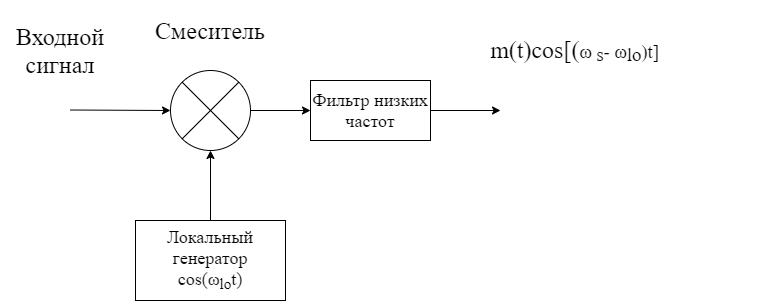
\includegraphics[width=\linewidth]{images/когеретное.png}
    \caption{Структурая схема гомодинного приема}
    \label{fig:homodyne det lit}
\end{figure}

Интенсивность в случае гомодинного детектирования будет описываться следующим выражением
\begin{equation}
    I(t) =|E(t)|^2 =  |E_1|^2 + |E_2|^2 + 2|E_1|\cos[(\omega_1 - \omega_2)t + \phi_1 - \phi_2]
\end{equation}\label{eq: fiedl homodyne}, где $E_1, E_2$ - комплексные амплитуды сигналов информационного и локального осциллятора, $\omega_1, \omega_2$ - частоты информационного сигнала и ЛО, $\phi_1, \phi_2$ - фазы информационного сигнала и ЛО. 
Но так как в случае гомодинного детектирования частоты излучения равны, то результат детектирования приводится к виду 
\begin{equation}
    S(t) = S_0 + S_m\cos(\Delta\phi)
\end{equation}
Таким образом результат интерференции при гомодинном детектировании пропорционален разности фаз между локальным осциллятором и исследуемым сигналом. Однако при $\Delta\phi = 90$ градусов невозможно однозначно различить фазу информационного сигнала и требуется дополнительные технические средства.  
\subsection{Гетеродинное детектирование}\label{sec:ch1/sect3/heterodyne lit}
Другой разновидностью когерентного  детектирования является гетеродинное детектирование. Данный метод нашел свое широкое распространение в радиотехнике c 1917 года под названием супергетеродинный приемник.
\begin{figure}
    \centering
    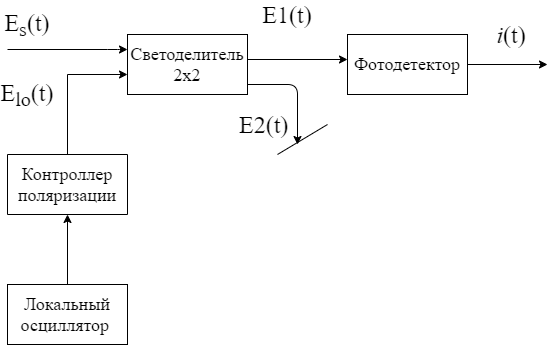
\includegraphics[width=\linewidth]{images/гетеродин для обзора.png}
    \caption{Стурктурная схема гетеродинного оптического приемника}
    \label{fig:heterodyne scheme lit}
\end{figure}
Суть данного метода заключается в следующем. Входной сигнал, несущий информацию подается на один из входов смесителя. На второй же вход смесителя подается сигнал локального осциллятора. При этом частоты входного сигнала и ЛО отличаются. В результате эти два сигнала интерферируют и на выходе смесителя образуется новая частота - промежуточная частота, которая равна разности частот ЛО и входного сигнала. Данный метод описывается следующим образом:
\begin{equation}
    I(t) =|E(t)|^2 =  |E_1|^2 + |E_2|^2 + 2|E_1|\cos[(\omega_1 - \omega_2)t + \phi_1 - \phi_2]
\end{equation}\label{eq: fiedl heterodyne}, где $E_1, E_2$ - комплексные амплитуды сигналов информационного и локального осциллятора, $\omega_1, \omega_2$ - частоты информационного сигнала и ЛО, $\phi_1, \phi_2$ - фазы информационного сигнала и ЛО. 
В результате на выходе фотоприемника формируется сигнал 
\begin{equation}
    S(t) = S_0 + S_m\cos((\omega_1 - \omega_2)t + \Delta\phi)
\end{equation}\label{eq:het result lit}
В выражении \ref{eq:het result lit} присутствует разностная частота $\omega_1 - \omega_2$, которая содержит себе информацию от входного сигнала о его амплитуде и фазе. Благодаря этому, возможно извлекать информацию из сложных типов модуляции, таких как квадртатурно-амплитудная, при этом не прибегая к дополнительным техническим приспособлениям. Данный метод детектирования сигналов является самым гибким для регистрации любых типов модуляции, однако требует точной подстройки частоты и ее стабилизации и фазовой синхронизации между входным сигналом и ЛО для проведения измерений фазы входного сигнала. 
\subsection{90-градусный оптический гибрид }\label{sec:ch1/sect3/90 hybrid lit}
Одним из главных недостатков гомодинного детектирования, описанного в разделе \ref{sec:ch1/sect3/homodyne lit} - является невозможность измерения сигнала с фазой в неортогональном состоянии относительно локального осциллятора. В результате этого при использовании 4 фазовых состояний для кодирования информации, 50 процентов из них будут утеряны из-за невозможности однозначно различить.
Для устранения этого существенного недостатка был разработан метод когерентного детектирования с использованием 90-градусного оптического гибрида или двойного гомодинирования. Данный метод развивает схему гомодинного детектирования из раздела \ref{sec:ch1/sect3/homodyne lit}. Входной сигнал и сигнал ЛО разделяются пополам на двух разных делителях. После этого части входного сигнала смешиваются с частями ЛО. Но в одном из плеч локального осциллятора установлен дополнительный фазовый сдвиг на $\frac{\pi}{2}$. За счет этой модификации возможно измерение фазы принятого сигнала во всех используемых состояниях. Результат измерения попадает на 2 балансный приемника или классических  фотодиода. В результате в том плече, где базисы фаз совпали, сигнал на выходе балансного детектора будет изменяться в зависимости от разности фаз. В другом же плече будет наблюдаться средний уровень сигнала, который невозможно интерпретировать как одно из измеренных фазовых значений. 
Данный метод приема лишен недостатка гомодинного приемника, однако он вносит дополнительные 3 дБ потерь по входному сигналу, что ухудшает его соотношение сигнал - шум, а также удваивает оптическую схему, что негативно сказывается на цене данного метода. Однако такой метод является более предпочтительным, чем одиночный гомодинный приемник. 
\section{Протоколы квантового распределения ключа на непрерывных переменных}\label{sec:ch1/CV-QKD review}
В качестве альтернативы КРК-ДП протоколам, которые в идеале основаны на однофотонном детектировании, КРК-НП \cite{braunstein2005} протоколы кодируют квантовые состояния в непрерывных переменных (НП) лазерного излучения, которые могут быть измерены с помощью гомодинного детектирования с ограниченным уровнем дробового шума. В гомодинном детекторе оптический сигнал подключается к сильному излучению локального осциллятора (ЛО) с ограниченным уровнем шума на сбалансированном делителе луча, и измеряется интенсивность света на выходных портах. В зависимости от разности оптических фаз между сигналом и ЛО, разность фототоков, возникающих в каждом из двух детекторов, будет пропорциональна одной из двух квадратур поля. Таким образом, ЛО несет в себе опорную фазу, которая позволяет переключаться между измерением q- и p-квадратур (или, в более общем случае, выполнять томографию состояния путем измерения функции Вигнера, связанной с состоянием).
Первое предложение об использовании квадратур бозонического поля для реализации КРК появилось в 1999 году, когда Ральф \cite{ralph1999} рассмотрел кодирование ключевых битов с помощью четырех фиксированных квадратурных смещений ярких когерентных или двухмодовых запутанных пучков. Позже Ральф обсудил безопасность двухмодовой схемы на основе запутанности более подробно \cite{ralph2000}, рассматривая не только атаки перехвата-передачи, но и телепортацию НП. Последняя была определена как оптимальная атака на протокол, накладывающая требования высокого сжатия сигнала и низких потерь в канале. Независимо от этого Хиллери \cite{hillery2000} предложил протокол КРК-НП, основанный на квадратурном кодировании одномодового луча, случайным образом сжатого в одном из квадратурных направлений. Безопасность от атак перехвата-передачи и расщепления луча оценивалась на основе принципа неопределенности. Другая ранняя схема КРК-НП была предложена Ридом \cite{reid2000} и основывалась на проверке корреляций типа ЭПР для обнаружения подслушивающего устройства.
В 2000 году Серф и другие \cite{cerf2001} предложили первый полностью непрерывный протокол КРК, в котором квадратуры сжатого луча использовались для кодирования безопасного ключа с гауссовским распределением. Безопасность протокола была показана против индивидуальных атак на основе соотношения неопределенностей и оптимальности квантового клонирования. Позже были введены процедуры согласования для гауссовски распределенных данных, что позволило реализовать исправление ошибок (ИО) и усиление секретности (УС)  близко к теоретическим границам \cite{vanassche2004}. Другой протокол КРК-НП, основанный на гауссовой модуляции сжатых пучков, был предложен Готтесманом и Прескиллом \cite{gottesman2001}. Было показано, что этот протокол защищен от произвольных атак при возможных уровнях сжатия, благодаря использованию квантовых кодов с коррекцией ошибок. В 2001 году Гроссханс и Гранжье представили основополагающий протокол с когерентным состоянием и гауссовской квадратурной модуляцией и показали его защищенность от индивидуальных атак \cite{grosshans2002}, прибегнув к НП-версии теоремы об отсутствии клонирования \cite{grosshans2001}. Стандартный протокол, основанный на прямой сверке (ПС), где Алиса является опорной стороной для постобработки информации, был, однако, ограничен 50-процентным пропусканием канала, то есть 3 дБ. В качестве попытки преодолеть ограничение в 3 дБ Зильберхорн и др. предложили использовать постселекцию в КРК-НП \cite{silberhorn2002}. В качестве альтернативы было показано, что использование обратной сверки (ОС), где опорной стороной является Боб, позволяет протоколу с когерентным состоянием быть защищенным от индивидуальных атак вплоть до произвольно низких коэффициентов пропускания канала \cite{grosshans2002a}. В 2004 году для протоколов с когерентным состоянием было предложено использование гетеродинного обнаружения \cite{weedbrook2004}; преимущество этого протокола без переключения заключается в том, что измеряются обе квадратуры, что увеличивает скорость передачи ключа. Безопасность КРК-НП от коллективных гауссовых атак была продемонстрирована независимо друг от друга Наваскуэсом и другими \cite{navascus2006} и Гарсией-Патроном и Серфом \cite{GarciaPatron2006}. Коллективные гауссовские атаки были полностью охарактеризованы Пирандолой и другими \cite{pirandola2008}, которые позже вывели мощности секретных ключей для КРК-НП \cite{pirandola2017,pirandola2009}. Безопасность от коллективных атак была расширена на общие атаки Реннером и Цираком \cite{renner2009} с помощью квантовой теоремы де Финетти, примененной к бесконечно-мерным системам. Это позволило завершить доказательства безопасности основных односторонних протоколов КРК-НП в асимптотическом пределе бесконечно больших наборов данных, в том числе с доверенным шумом \cite{pirandola2014, usenko2016, laudenbach2019}. Следующим развитием стало изучение эффектов конечного размера и полностью композитных доказательств. Стоит также упомянуть о существовании других направлений исследований, в которых при вычислении скорости секретного ключа учитываются ограничения реалистичного подслушивающего устройства \cite{hosseinidehaj2019, pan2020}.
В следующих разделах, помимо стандартных односторонних гауссовских протоколов (основанных на когерентных или сжатых состояниях), рассмотрим двусторонние протоколы, протоколы тепловых состояний, одномерные  протоколы, протоколы с дискретной модуляцией и протоколы с ретрансляцией, такие как КРК-НП НПУ. Понятно, что это не охватывает все современные разработки в широкой области КРК-НП. Например, здесь  явно не обсуждаются протоколы, основанные на использовании негауссовых операций, таких как вычитание фотонов \cite{guo2017}, квантовый катализ \cite{guo2019} или квантовые ножницы \cite{ghalaii2020}.


\subsection{Протокол квантового распределения ключа с использованием модуляции Гаусса}\label{sec:ch1/sect4/GG02}
Протокол квантового распределения ключа на непрерывных переменных с применением Гауссовой модуляции является одним из первых протоколов, для которого существует доказательство секретности с учетом эффектов конечного ключа и против оптимальной атаки злоумышленника. С учетом этого факта и того, что его реализация может быть достаточно простой, данный протокол стал одним из первых реализованных на практике протоколом на непрерывных переменных. 
\subsubsection{Этапы протокола с использованием модуляции Гаусса}
Данный протокол состоит из 4 шагов - 1. подготовка и распределение состояний, 2. - сверка ошибок, 3. определение параметров и 4. усиление секретности. 
\begin{enumerate}
    \item Подготовка и распределение состояний: Алиса готовит большое количество когерентных состояний $\ket{\alpha_1} \dots \ket{\alpha_N} $, где $\alpha_i$ независимые и тождественно распределенные комплексные гауссовские переменные распределением $V_0$. В зависимости от протокола (гомодинный или гетеродинный) Боб измеряет либо случайную квадратуру (x или p) для каждого состояния и сообщает Алисе о своем выборе, либо обе квадратуры. Затем Боб получает список из N или 2N вещественных чисел, соответствующих результатам его измерений. Алиса также имеет доступ к своему собственному списку данных (она хранит только соответствующие значения квадратур, если Боб зарегистрировал сигналы с помощью гомодинным детектированием). Обозначим соответствующие списки Алисы и Боба через  $x = {x_1 \dots x_n}$ и $y = {y_1 \dots y_n}$, (где n - N или 2N).
    \item Исправление ошибок: Протокол в целом достигает лучшей производительности при обратном согласовании : это означает, что строка Боба соответствует необработанному ключу, а Алиса пытается угадать его значение. Для достижения этой цели Алиса и Боб используют классические методы исправления ошибок. Точнее, Алиса и Боб договариваются о линейном коде с коррекцией ошибок до начала протокола, и Боб отправляет Алисе значение синдрома y для этого кода. Чтобы восстановить y, Алисе нужно просто исправить x, то есть декодировать в косетевой код, определяемый полученным синдромом. 
    \item Оценка параметров: Этот шаг полезен для получения верхней границы информации, доступной Еве. Для протоколов КРК-НП это обычно требует оценки ковариационной матрицы двухстороннего состояния, разделяемого Алисой и Бобом. Получив эту оценку, Алиса и Боб могут вычислить размер $\ell$ безопасного ключа, который они могут извлечь из своего состояния.
    \item Усиление конфиденциальности: Алиса и Боб применяют случайную универсальную хэш-функцию к своим соответствующим (исправленным) строкам и получают две строки $S_A$  и $S_B$ длины $\ell$.
\end{enumerate}
Варианты этого протокола могут отличаться типом подготавливаемых состояний (когерентные, сжатые или даже тепловые) и способом детектирования (гомодинный или гетеродинный), но основные этапы протокола остаются в основном идентичными

\subsubsection{Экспериментальная реализация протокола с модуляцией Гаусса} \label{GG02 exp lit}
Как и в случае КРК на дискретных переменных, протоколы КРК-НП "приготовление и измерение" в целом проще реализовать на практике \cite{diamanti2015}. Далее подробно описывается реализация протокола GG02 \cite{grosshans2002}, принцип и безопасность которого были рассмотрены в разделах 2 и 3 соответственно, с помощью волоконной оптики. Этот протокол особенно интересен с практической точки зрения \cite{fossier2009}, поскольку он требует всего лишь генерации когерентных состояний, их модуляции в фазовом пространстве и обнаружения квадратур полученных состояний с помощью гомодинных (или гетеродинных) методов. Компоненты, необходимые для достижения этих функциональных возможностей, легко доступны на телекоммуникационной длине волны, которая подходит для работы с волоконно-оптическими системами. Оптическая конфигурация для выполнения этого протокола показана на рисунке \ref{fig:gg02 lit}.
\begin{figure}
    \centering
    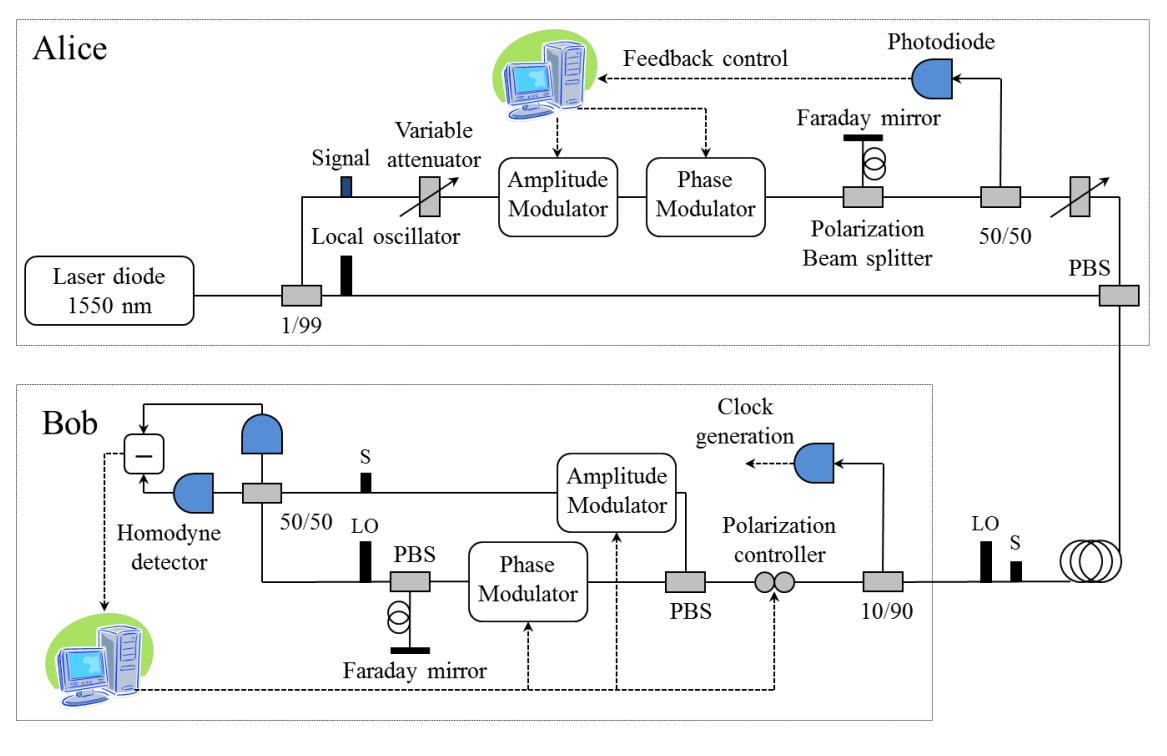
\includegraphics[width=\linewidth]{images/gg02 lit.png}
    \caption{Оптическая схема волоконной системы КРК-НП с гомодинным детектированием. Laser diode - лазерный диод, signal - сигнал, Local oscillator - локальный осциллятор, Variable attenuator - переменный аттенюатор, Amplitude modulator - амплитудный модулятор, Phase modulator - фазовый модулятор, Polarization beam splitter (PBS) - поляризационный делитель луча, Faraday mirror - Зеркало Фарадея, Photodiode - Фотодиод, Feedback control - управление обратной связью, Polarization controller - контроллер поляризации, Clock generation - генерация опорной частоты, Homodyne detector - гомодинный приемник.}
    \label{fig:gg02 lit}
\end{figure}
В этой схеме сигнал и опорная фаза (или локальный осциллятор), необходимые для выполнения когерентного обнаружения, генерируются источником лазерного диода в месте нахождения Алисы. Сигнал модулируется по амплитуде и фазе в соответствии с гауссовским распределением, как того требует протокол, а затем ослабляется на подходящем уровне дисперсии модуляции. Он также мультиплексируется по времени и по поляризации с локальным осциллятором перед входом в квантовый канал. На месте Боба два сигнала демультиплексируются с помощью линии задержки и поляризационного делителя луча и накладываются во времени для интерференции на ограниченный шумами сбалансированный импульсный гомодинный детектор. Квадратурная селекция, требуемая протоколом GG02, выполняется фазовым модулятором, помещенным в тракт локального генератора. Установка дополнена несколькими активными элементами обратной связи и управления, которые обеспечивают необходимые условия синхронизации и стабильности для выполнения квантового распределения ключей. 
Описанная система реализует первую часть, а именно (1) распределение и измерение состояния, полного протокола GG02, описанного в разделе \ref{GG02 exp lit}; остальные части постобработки, а именно 2 согласование ошибок, 3 оценка параметров и 4 усиление конфиденциальности, и, в частности, первые две, требуют сложных вычислительных алгоритмов. Первоначальная реализация оптической установки на рисунке \ref{fig:gg02 lit} использовалась в европейской сети SECOQC QKD, которая была развернута по проложенным оптическим волокнам и объединяла различные технологии КРК. Она также использовалась в полевых испытаниях линии связи точка-точка с классическим симметричным шифрованием и быстрым обновлением ключей, обеспечиваемым квантовым слоем, которые продемонстрировали надежность работы системы КРК-НП в течение длительного периода времени в условиях серверной. Эти реализации, а также некоторые другие, были пригодны для защиты коммуникаций в сетях городского масштаба (с расстоянием до 25 км) с высокими требованиями к скорости передачи данных. Хотя существует несколько интересных применений экспериментов на коротких расстояниях, с точки зрения квантовых информационных сетей важно иметь возможность увеличить расстояние связи за этот предел. В реализациях дискретно-переменного КРК ограничение по расстоянию в основном определяется характеристиками однофотонных детекторов, в частности, их темновыми отсчетами. В КРК-НП ограничение дальности было связано с эффективностью сложных методов постобработки. Хотя это уже не так, полезно понять причину этого ограничения: эффективное согласование коррелированных гауссовских переменных на самом деле затруднено, особенно при низких отношениях сигнал/шум (SNR), которые присущи экспериментам на больших расстояниях, что снижает коэффициент эффективность сверки. 
Помимо исправления ошибок, процедура оценки параметров также имеет решающее значение для извлечения секретного ключа на практике. Для оптической установки на рисунке \ref{fig:gg02 lit} соответствующими экспериментальными параметрами являются дисперсия модуляции Алисы $V_A$, коэффициент пропускания канала T и избыточный шум $\xi$, который представляет собой шум, добавляемый каналом сверх основного шума выстрела, и соответствует обычному коэффициенту ошибок квантового бита, встречающемуся в дискретно-переменных реализациях КРК. Как $V_A$, так и $\xi$ обычно выражаются в единицах дробового шума. Параметр $V_A$ подстраивается в реальном времени, чтобы в любой момент времени быть как можно ближе к SNR, соответствующему порогу доступного кода с исправлением ошибок, в то время как параметры T и $\xi$ должны оцениваться в реальном времени путем случайного раскрытия части ключа. Два дополнительных экспериментальных параметра, которые используются для вычисления оценки секретной информации, которая может быть извлечена из общих данных, - это скорость электронного шума и эффективность $\eta$ обнаружения гомодина. В так называемом реалистичном сценарии КРК-НП предполагается, что эти параметры недоступны для Евы и измеряются в ходе безопасной процедуры калибровки, которая проводится перед развертыванием системы. Однако в общем случае эти параметры могут быть доступны Еве. Процедура оценки параметров позволяет вычислить границы для информации подслушивающего лица, принимая во внимание неопределенность калиброванных значений.

\subsection{Протокол квантового распределения ключа с использованием модуляции Гаусса и локальным осциллятором, сгенерированным на приемной стороне}\label{sec:ch1/sect4/subsec2} %Generating the local oscillator locally in continuous-variable quantum key
%distribution based on coherent detection
Как протоколы КРК на дискретных переменных  (КРК-ДП) , основанные на обнаружении одиночных фотонов \cite{bennett1984,ekert1991}, так и протоколы КРК на непрерывных переменных (КРК-НП), основанные на когерентном детектировании \cite{ralph1999,hillery2000,grosshans2002} были продемонстрированы как жизнеспособные решения на практике. Одним из известных протоколов КРК-НП является протокол когерентного состояния с гауссовской модуляцией (ГМКС) \cite{grosshans2002}, который был продемонстрирован на 80-километровой оптоволоконной  линии связи \cite{jouguet2013a}. Одним из важных преимуществ ГМКС КРК  является его устойчивость к некогерентному фоновому шуму. Сильный локальный осциллятор (ЛО), используемый в когерентном обнаружении, также действует как естественный и чрезвычайно селективный фильтр, который может эффективно подавлять шумовые фотоны. Эта внутренняя функция фильтрации делает КРК-НП привлекательным решением для безопасного распределения ключей по зашумленному каналу, таком как освещенное волокно в обычной оптоволоконной оптической сети \cite{kumar2015} или оптической линии связи в свободном пространстве \cite{heim2014}.
Однако все существующие реализации КРК-НП основанные на когерентном детектировании, имеют серьезный недостаток: для уменьшения фазового шума как сигнал, так и ЛО генерируются одним и тем же лазером и распространяются по небезопасному квантовому каналу \cite{grosshans2002, jouguet2013a, heim2014} 1. Такая схема имеет несколько ограничений. Во-первых, она позволяет Еве получить доступ как к квантовому сигналу, так и к ЛО. Ева может проводить сложные атаки, манипулируя ЛО, что было продемонстрировано в недавних исследованиях \cite{ma2013, huang2013,jouguet2013}. Во-вторых, Передача сильного ЛО по каналу с потерями может резко снизить эффективность КРК в некоторых приложениях. Например, для достижения когерентного обнаружения с ограничением по дробовому шуму необходимое число фотонов в ЛО обычно превышает $10^8$ фотонов на импульс на стороне приемника. При частоте повторения импульсов 1 ГГц и потерях в канале 20 дБ, требуемая мощность ЛО на входе квантового канала составляет около 1,2 Вт (на длине волны 1550 нм). Если оптическое волокно используется в качестве квантового канала, шумовые фотоны, генерируемые сильным ЛО внутри оптического волокна, могут значительно снизить эффективность КРК и пропускную способность мультиплексирования. В-третьих, ЛО обычно на 7 или 8 порядков ярче, чем квантовый сигнал, поэтому требуются сложные схемы мультиплексирования и демультиплексирования для эффективного отделения ЛО от квантового сигнала на стороне приемника.
В КРК-НП желательно генерировать ЛО 'локально', используя независимый лазерный источник на стороне приемника. К сожалению, такая схема никогда не была реализована на практике. Основная проблема заключается в том, как эффективно установить надежную фазовую привязку между Алисой и Бобом. Хотя в классической когерентной связи были разработаны различные методы, такие как восстановление несущей \cite{ip2007}, оптическая фазовая автоподстройка частоты \cite{ma2013}, и оптическая инжекционная фазовая подстройка частоты \cite{fice2011}, были разработаны для классической когерентной связи, но эти методы не подходят для КРК, где квантовый сигнал крайне слаб, а допустимый фазовый шум мал.
Кроме того, чтобы предотвратить манипуляции Евы с ЛО, лазер ЛО должен быть изолирован от внешнего мира как оптически, так и электрически.
В этой статье решается вышеупомянутая давно нерешенная проблема, предложив и продемонстрировав схему восстановления данных с помощью пилота схема восстановления данных с обратной связью, которая обеспечивает надежное когерентное обнаружение с использованием "локально" генерируемого ЛО.
Эта схема основана на наблюдении, что в ГМКС КРК, Бобу не нужно выполнять измерение в "правильном базисе". Фактически, Боб может выполнить измерение в произвольно повернутом базисе, поскольку при условии, что информация о базисе (фазовый эталон) если информация о базисе (фазовый эталон) доступна после измерения. Имея эту информацию  после измерения, Алиса или Боб могут вращать имеющиеся данные и генерировать коррелированные данные с другими. 
\subsubsection{Экспериментальная реализация протокола КРК на непрерывных переменных с модуляцией Гаусса.}
\begin{figure}
    \centering
    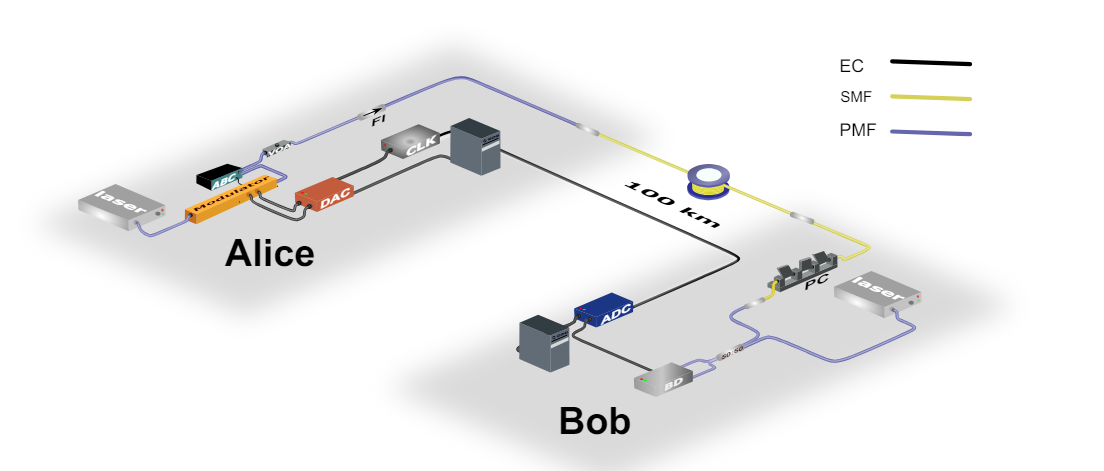
\includegraphics[width=0.9\linewidth]{images/QKD CV LLO.png}
    \caption{Станция Алисы состоит из непрерывного (CW) лазера, работающего на длине волны 1550 нм, синфазного и квадратурного (IQ) модулятора с автоматическим регулятором смещения (ABC) для получения когерентных состояний на боковых частотах. A Для управления IQ-модулятором использовался цифро-аналоговый преобразователь (ЦАП) с разрешением 16 бит и частотой дискретизации 1 Гвыб/с. Переменный оптический аттенюатор (VOA) использовался после IQ-модулятора для регулировки дисперсии модуляции квантового сигнала. Изолятор Фарадея (ФИ), направление которого указано стрелкой, используется перед 100-километровым оптоволоконным каналом со сверхнизкими потерями, который представляет собой квантовый канал. Станция Боба состоит из поляризационного контроллера (ПК) для настройки поляризации входящего сигнала и сбалансированного светоделителя для наложения этого сигнала на локальный осциллятор, генерируемый другим CW-лазером (разблокированным/свободно работающим по отношению к лазеру Алисы). Сигнал был обнаружен и оцифрован с помощью сбалансированного детектора (BD), а затем аналого-цифрового преобразователя (АЦП) с частотой дискретизации 1 Гвыб/с.}
    \label{fig:CV QKD ЛЛО lit}
\end{figure}
На рисунке \ref{fig:CV QKD ЛЛО lit} показана оптическая схема  системы КРК-НП с "локальным" локальным осциллятором (ЛЛО) \cite{hajomer2024}, основанной на протоколе когерентного состояния с гауссовской модуляцией. У отправителя, Алисы, в качестве оптического носителя использовался непрерывный лазер (CW) с узкой шириной линии $\approx$ 100 Гц, работающий на длине волны 1550 нм. Когерентные состояния готовились путем модуляции КВ-лазера с помощью синфазно-амплитудного (IQ) модулятора, управляемого 16-битным цифро-аналоговым преобразователем (ЦАП) с двумя каналами, работающими с частотой дискретизации 1 Гвыб/с. IQ-модулятор работал в однополосном режиме, управляя напряжениями смещения постоянного тока (DC) с помощью автоматического регулятора смещения (ABC). После IQ-модулятора был установлен переменный оптический аттенюатор (VOA) для регулировки дисперсии модуляции теплового состояния. На выходе отправителя был добавлен изолятор Фарадея, чтобы избежать обратных отражений от канала и атак "троянского коня". Сигнал передавался по квантовому каналу, изготовленному из коммерческого волокна с ультранизкими потерями (TeraWave SCUBA 150 Ocean Optical Fiber). Затухание волокна составляет 0,146 дБ/км на длине волны 1550 нм. Общие потери в нашем 100-километровом оптоволоконном канале составили 15,4 дБ из-за разницы диаметров модового поля между соединением волокна SMF-28 и SCUBA 150.
В приемнике Боба для измерения квантового состояния использовалось радиочастотное (РЧ) гетеродинное детектирование. Для этого в качестве ЛЛО использовался другой CW-лазер, свободно работающий по отношению к лазеру Алисы. Разница частот между
лазерами Алисы и Боба составляла $\approx$ 230 МГц. Затем поляризация квантового сигнала была настроена так, чтобы соответствовать поляризации ЛЛО с помощью регулятора поляризации. Затем квантовый сигнал и ЛЛО были объединены на сбалансированном светоделителе,
затем самодельный сбалансированный детектор с полосой пропускания
$\approx$ 365 МГц для обнаружения интерференционной картины. Наконец, обнаруженный сигнал оцифровывался с помощью 16-битного аналого-цифрового преобразователя (АЦП) с частотой дискретизации 1 Гвыб/с и записывался для автономной цифровой обработки сигнала. АЦП и ЦАП были синхронизированы с помощью опорного генератора (CLK) с частотой 10 МГц.
Время измерения делилось на кадры, каждый из которых содержал $10^7$ выборок АЦП. Три измерения проводились автономно: измерение квантового сигнала, измерение вакуумного шума (лазер Алисы выключен, лазер Боба включен) и измерение электронного шума (лазер Алисы выключен, лазер Боба выключен). Выигрыш вакуумного шума по сравнению с электронным составил $\approx$ 15 дБ в полосе частот квантового сигнала. Чтобы откалибровать $V_{mod}$ теплового состояния, проводились измерения "спина к спине" (B2B), в которых Алиса и Боб были соединены через короткий волоконный патч-корд, а VOA был тонко настроена для установки различных значений $V_{mod}$.
\newline Передача данных на большие расстояния является ключевым требованием для широкомасштабного развертывания и интеграции КРК в существующие телекоммуникационные сети. КРК-НП естественным образом подходит для такой интеграции. Однако безопасная и практичная конфигурация системы (ЛЛО КРК-НП) сталкивается с ограничениями по дальности передачи из-за фазового
фазового шума лазеров. В данной работе демонстрируется  возможность передачи данных на большие расстояния ЛЛО КРК-НП по оптоволоконному каналу длиной 100 км . Этот рекордный эксперимент стал возможен благодаря использованию машинного обучения для компенсации фазового шума и оптимизации модуляции для согласования информации и избыточного шума одновременно.

\section{Фазовый шум в системах квантового распределения ключа}\label{sec:ch1/sect5}
Фазовый шум в системах квантового распределения ключа является одним из факторов, которые ограничивают скорость выработки секретного ключа. В то время, как этот эффект практически не влияет на протоколы, построенных на дискретных переменных, но этот эффект является критическим для протоколов на непрерывных переменных, как и для протоколов, основанных на "полях близнецах" и с недоверенным приемным узлом. В случае этих протоколов происходит интерференция либо нескольких когерентных состояний между собой, либо между когерентным состоянием и локальным осциллятором. В обоих случаях происходит измерение, которое будет зависеть от разности фаз между взаимодействующими компонентами излучения. И в случае наличия дополнительного фазового шума, результат этой интерференции будет абсолютно случайным, независимым от закодированных состояний Алисой и Бобом. В этом случае ключ не будет сгенерирован. Поэтому данный шум необходимо компенсировать различными методами.
\newline Избыточный шум в системах КРК может быть обусловлен различными источниками: дискретизация, модуляция, относительный шум интенсивности (RIN), рассеяние Рамана и  остаточный фазовый шум (RPN). Предполагается, что эти источники шума статистически независимы и поэтому общий избыточный фазовый шум может быть представлен в виде суммы независимых величин
\begin{equation}
    \zeta = \zeta_{RIN} + \zeta_{mod} + \zeta_{quant} + \zeta_{Ramman} + \zeta_{RPN} + K
\end{equation}\label{eq:noise lit}
Среди этих источников шума, остаточный фазовый шум (ОФШ), определяется как распределение разности между реальной фазой квантового сигнала и измеренной фазой принятого сигнала, является главным источником избыточного шума в системах КРК-НП ЛЛО. В случае гауссово-модулированного протокола на когерентных состояния, избыточный шум, связанный с ОФШ на приемной стороне определяется как 
\begin{equation}
    \zeta_{ОФШ} = 2TV_{mod}(1-e^\frac{-V_{RPN}}{2}) 
\end{equation}\label{eq: noise phase llo lit}, где T - пропускание, включающее в себя квантовый канал и эффективность детектора, $V_{mod}$ - распределение модуляции, т.е. распределение ансамбля когерентных состояний и $V_{ОФШ}$ - распределение остаточного фазового шума.
Исходя из выражения \ref{eq: noise phase llo lit}, доступно два варианта уменьшение фазового шума в КРК-НП с ЛЛО: работа системы при низкой дисперсии модуляции или минимизация ОФШ. Хотя первый вариант практичен и прост в реализации, он требует тщательной оптимизации $V_{mod}$ из-за зависимости скорости выработки секретного ключа от дисперсии модуляции. В частности, от дисперсии модуляции зависят как взаимная информация, так и эффективность согласования информации.
Для уменьшения ОФШ требуется эффективная оценка фазы. В настоящее время стандартный подход заключается в использовании пилотных методов для оценки относительной фазы между непрерывно излучающими лазерами  передатчика и приемника. Качество оценки фазы сильно зависит от отношения сигнал/шум (SNR) пилотных сигналов, реализуемых с помощью одночастотных тонов или обучающих символов, передаваемых вместе с квантовым сигналом. Однако эти методы ограничены потерями в канале, которые увеличиваются с расстоянием, и необходимостью в маломощном пилотном сигнале для уменьшения перекрестных помех квантовому сигналу.

\subsection{Методы борьбы с фазовым шумом в системах квантового распределения ключа}\label{sec:ch1/sect5/subsec1}
В ходе развития технологии квантового распределения ключа были разработаны несколько методов компенсации фазовых искажений с целью улучшения характеристик конечных систем. Существует несколько способов реализации компенсаций фазовых искажений: восстановление фазы несущей частоты, пилотные импульсы и реализация обратной связи в виде оптической инжекции или оптической фазовой автоподстройки частоты. Данные методы обладают как своими преимуществами, так и недостатками. Данный раздел посвящен рассмотрению принципов работы данных методов компенсации фазовых искажений. 
\subsubsection{Пилотные импульсы}Первым из методов восстановления стали так называемые пилотные импульсы \cite{wang2020}. Их суть заключается в том, что к квантовым состояниям мультиплексируется дополнительный классический сигнал, который является опорным для измерения фазового шума при прохождении квантового канала. После прохождения этими сигналов квантового канала, они попадают на схему демультиплексирования и разделяются. На балансном детекторе происходит измерение фазы и пилотного импульса, и квантового сигнала. Так как эти оба сигнала распространялись по одному и тому же каналу, а также были излучены одним и тем же источником, то их фазовые шумы являются скоррелированными. В результате измерения фазы  пилотного импульса, можно вносить корректировки измеренного фазового набега в квантовом сигнале на этапе постобработки. 
\newline Однако данный метод усложняет приемный модуль за счет необходимости дополнительной системы демультиплексирования, а также увеличивает шум, связанный с рассеянием, так как передаваемый  пилотный импульс должен быть достаточно мощным для точных измерений.
\subsubsection{Оптическая фазовая автоподстройка частоты}
Другим же методом подстройки фазы двух источников излучения является оптическая фазовая автоподстройка частоты или ОФАПЧ (OPLL) \cite{khaksar2023}. В этом случае, два лазера сбиваются на фотоприемнике. Их разностная частота подстраивается так, чтобы она сравнялась с опорной частотой генератора, относительно которой будет подстраиваться фаза излучения. 
В качестве источника опорной частоты может выступать термостатированный кварцевый генератор. Эти частоты сбиваются на смесителе для формирования сигнала ошибки. Этот сигнал ошибки передается на PID контроллер температуры лазера для управления его длиной волны до тех пор, пока этот сигнал ошибки не станет меньше заданного значения.
Из плюсов данной реализации можно выделить ее точность и скорость работы. К недостаткам можно отнести сложность исполнения и необходимость точной подстройки и стабилизации температур и токов лазеров.

\section{Известные атаки злоумышленника на источники лазерного излучения}\label{sec:ch1/sect7}
Секретность распределенного ключа в системах квантового распределения базируется на теоретических доказательствах секретности, в которых допускается, что злоумышленник (Ева) может сделать все, что не запрещено законами квантовой физики. Однако, несовершенства технической реализации систем КРК позволяют Еве их использовать для доступа к части секретного ключа. Среди таких атак выделяется атаки на источник лазерного излучения в системе КРК. Этот тип атак позволяет увеличить мощность, излучаемую лазером, установленным в Алисе, и таким образом увеличить среднее число фотонов. Этот эффект позволяет применять атаку с расщеплением числа фотонов эффективнее и получать доступ к части секретного ключа. 
\newline Другой же тип атаки направлен непосредственно на Локальный осциллятор в системе КРК-НП для изменения времени начала синхронизации
\subsection{Атака "засевом" лазерным излучением}\label{sec:ch1/sect7/subsec1}
Первоначально атаки злоумышленника были нацелены на приемную часть, а именно на детектор одиночных фотонов \cite{makarov2009, sajeed2020, chistiakov2019, qian2018}. В результате этой атаки злоумышленник имеет возможность "навязывать" секретный ключ легитимным пользователям \cite{lydersen2010}. 
В дальнейшем  появились атаки на модуляторы - атака "троянским конем". Такое воздействие позволяет узнать о выборе базиса легитимными пользователями и иметь доступ к секретному ключу за счет зондирования фазового модулятора излучением, сильно отличающимся по длине волны от той, что используют Алиса и Боб \cite{jain2014,a-etsi2021,gisin2006}.
Но существует и атака на источник излучения из состава системы квантового распределения ключей - атака "засевом" лазерным излучением \cite{huang2019,lovic2023}. Одним из главных условий секретности распределенного ключа в системах КРК является предположение, что интенсивность квантовых состояний, передаваемых Алисой, в среднем меньше 1 фотона на импульс.
Однако атака "засевом" позволяет нарушить это предположение. Стратегия этой атаки заключается в следующем. Злоумышленник использует свое мощное излучение на близкой длине волны и посылает его в оптическую схему Алисы.
В результате мощность, претерпевшая затухание из-за прохождения оптических элементов, попадает в резонатор лазера Алисы. Инжектированные таким образом носители увеличивают выходную мощность вынужденного излучения Алисы. 
Под действием излучения увеличивается и энергия импульса, и непрерывная мощность. В результате этого увеличивается излучаемое число фотонов Алисой. Этот эффект позволяет злоумышленнику либо производить различение состояний-ловушек в протоколах с их реализацией или же проводить успешнее атаку с разделением числа фотонов, тем самым получая доступ к секретному ключу. 
Еще одним эффектом, который негативно сказывается на секретности распределяемого ключа, является возможность злоумышленника вносить корреляции в излучение Алисы. Это происходит также с помощью атаки "засевом" лазерным излучением.
Однако создание корреляций происходит с помощью зондирования импульсным излучением, а не непрерывным как в других работах. Интерференционная картина импульсов злоумышленника и Алисы будут скоррелированны и для внесения этой корреляции не требуется большой мощности - достаточно 1 нВт средней мощности. 
С ростом зондирующей мощности корреляции будут только возрастать, что позволит получить Еве также доступ к части секретного ключа.
\newline Таким образом, атака "засевом" лазерным излучения является серьезной угрозой стойкости систем КРК, которую необходимо учитывать и разрабатывать контрмеры для ее предотвращения. 

\subsection{Атака на мощность локального осциллятора в системах квантового распределения ключа на непрерывных переменных}\label{sec:ch1/sect7/subsec2}
Существующие системы квантового распределения ключей на непрерывных переменных используют один лазер для генерации квантовых состояний и локального осциллятора. Такой подход позволяет упростить конечную систему. 
Однако, у генерации ЛО на стороне передатчика есть несколько недостатков: снижение уровня сигнала ЛО при передаче по волокну в виду естественного затухания. Другой же недостаток данного подхода - уязвимость ЛО ко внешнему воздействию злоумышленника.
В работе \cite{jouguet2013, fan2023} описывается атака на ЛО в системе КРКНП. В доказательствах секретности не учитывается ЛО, хотя он, как классический сигнал, может быть без проблем перехвачен, измерен, усилен и отправлен снова в канал.
Локальный же осциллятор используется для оценки пропускания канала и оценки распределения шума детектора - дробового шума. Эта величина является критической для оценки секретности ключа. 
Стратегия злоумышленника заключается в следующем. Злоумышленник вносит затухание в начало локального осциллятор. Так как ЛО используется для генерации опорной частоты, то внесение затухания в ЛО вызывает задержку во времени при формировании опорной частоты.
Для выполнения успешной атаки Ева производит следующие действия
\begin{enumerate}
    \item Нарушитель, Ева, вводит аттенюатор, не разрушающий фазу излучения, в квантовый канал и применяет некоторое затухание $\alpha$ ($0\leq \alpha \leq 1)$ на часть $\nu (0 \leq \nu \leq 1)$ импульсов локального осциллятора для изменения их формы. Тактовая частота, формируемая для гомодинного детектирования, зависящая от этих импульсов, сдвигается на величину $\delta$.
    \item Ева вводит светоделитель в квантовый канал и для части $\mu (0 \leq \mu \leq 1)$ входящих импульсов выполняет измерение обеих квадратур и подготавливает подходящие квантовые состояния, когда как для части $1 -\mu$ сигнальных импульсов, применяется функция светоделителя. Это называется частичной атакой "перехват - пересылка". 
\end{enumerate} 
Когда Ева увеличивает часть $\mu$ сигнальных импульсов, для которых она выполняет атаку "перехват-пересылка", то она вносит больше шума, который снижает количество секретных бит ключа, которые Алиса и Боб могут извлечь из квантовой передачи.
Часть $\nu$ локального осциллятора, в которую вносится затухание, и само затухание $\alpha$ - это два параметра, которые выполняют одну и ту же функцию - масштабируют распределение измерений, выполненных Бобом, не изменяя границу его дробового шума. Это приводит к тому, что Алиса и Боб приходят к выводу о том, что в квантовый канал не было внесено дополнительного шума, зеленый график на рисунке \ref*{fig:CV_attack} и поэтому распределяют ключ без обнаружения Евы.

\begin{figure}
    \centering
    \includegraphics*[width=\linewidth]{CV_attack.png}
    \caption{График распределения шума гомодинного детектора без атаки (красный цвет) и под действием атаки (зеленый) на ЛО.}
    \label{fig:CV_attack}
\end{figure}
\subsection{Выводы по главе}\label{sec:ch1/sect8}
В данной главе рассматриваются основы технологии квантового распределения ключей. Рассмотрены подходы по созданию систем КРК на дискретных переменных по топологии "точка-точка", так и с недоверенным приемным узлом. Как альтернатива протоколам на дискретных переменных рассмотрены протоколы на непрерывных переменных. Продемонстрированы  различные подходы к реализации локального осциллятора в системах КРКНП. Показаны этапы протокола выработки битовых последовательностей для протоколов на дискретных переменных, так и на непрерывных.
Изучен вопрос атак на техническую реализацию систем квантового распределения ключей. Особенно акцентировано внимание на атаках на источники излучения в КРК. Все рассмотренные вопросы создают базовое понимание технологии КРК, которые необходимы для понимания последующих глав.